\documentclass[t, 8pt]{beamer}  % [t] = top-align all frames

% --- Base ---
\useoutertheme[hideothersubsections, width=2.2cm]{sidebar}
\useinnertheme{default}
\usefonttheme{serif}
\usepackage{mathpazo}
\usepackage{microtype}
\usepackage[T1]{fontenc}
\usepackage{tikz}
\usetikzlibrary{arrows.meta, decorations.pathreplacing, positioning, fit, backgrounds, calc}
\usepackage{fontawesome5}
\usepackage{booktabs}
\usepackage{array}
\usepackage[normalem]{ulem}
\hypersetup{colorlinks=true, urlcolor=blue!60!black, linkcolor=.}
\tikzset{
  invisible/.style={opacity=0},
  visible on/.style={alt={#1{}{invisible}}},
  alt/.code args={<#1>#2#3}{\alt<#1>{\pgfkeysalso{#2}}{\pgfkeysalso{#3}}},
}

% --- Palette ---
\definecolor{paper}{RGB}{247, 243, 232}
\definecolor{sidebarbg}{RGB}{238, 233, 219}
\definecolor{codebg}{RGB}{240, 234, 217}
\definecolor{ink}{RGB}{26, 20, 10}
\definecolor{inkfaint}{RGB}{130, 118, 96}
\definecolor{inkghst}{RGB}{185, 175, 155}     % very faint, for rules
\definecolor{keyblue}{RGB}{61, 107, 140}
\definecolor{keyteal}{RGB}{61, 112, 104}
\definecolor{keyterra}{RGB}{139, 77, 42}
\definecolor{yellow}{RGB}{207, 133, 54}
\definecolor{green}{RGB}{108, 164, 82}

% exactblock: #1 = 0 (nothing underlined), 1 (global underlined), 2 (locals underlined)
\newcommand{\exactblock}[1]{%
  \begin{tikzpicture}[
    tok/.style={font=\ttfamily\fontsize{7}{9}\selectfont\color{ink}, inner sep=1.5pt},
    ann/.style={font=\fontsize{6}{6}\selectfont\color{inkfaint}},
  ]
    \node[tok] (exact) {exact};
    \node[tok, right=3pt of exact] (lem) {le\_of\_le\_of\_eq};
    \node[tok, right=15pt of lem] (h1) {h$_1$};
    \node[tok, right=5pt of h1] (ca) {(congrArg List.length (id (Eq.symm h$_2$)))};

    \draw[color=inkfaint, line width=0.5pt, decorate,
          decoration={brace, mirror, amplitude=4pt}]
      (lem.south west) -- (lem.south east);
    \node[ann, align=center, below=7pt of lem, font=\fontsize{6}{6}\selectfont\ifcase#1\relax\color{inkfaint}\or\color{inkfaint}\else\color{inkghst}\fi] (lbl1) {Global Search\\[2pt]%
      \ifcase#1\relax(DiscrTree)\or\setlength{\ULdepth}{3pt}\uline{(DiscrTree)}\else(DiscrTree)\fi};

    \draw[color=inkfaint, line width=0.5pt, decorate,
          decoration={brace, mirror, amplitude=4pt}]
      (h1.south west) -- (h1.south east);
    \node[ann, align=center, below=7pt of ca, font=\fontsize{6}{6}\selectfont\ifcase#1\relax\color{inkfaint}\or\color{inkghst}\else\color{inkfaint}\fi] (lbl3) {Local Search\\[2pt]%
      \ifcase#1\relax(SolveByElim)\or(SolveByElim)\else\setlength{\ULdepth}{3pt}\uline{(SolveByElim)}\fi};

    \draw[color=inkfaint, line width=0.5pt, decorate,
          decoration={brace, mirror, amplitude=4pt}]
      (ca.south west) -- (ca.south east);
    \node[ann, align=center, anchor=west, font=\fontsize{6}{6}\selectfont\ifcase#1\relax\color{inkfaint}\or\color{inkghst}\else\color{inkfaint}\fi] (lbl2) at ([xshift=-17pt]lbl3 -| h1.west) {Local Search\\[2pt]%
      \ifcase#1\relax(SolveByElim)\or(SolveByElim)\else\setlength{\ULdepth}{3pt}\uline{(SolveByElim)}\fi};

    \begin{scope}[on background layer]
      \node[fill=codebg, rounded corners=3pt, inner xsep=8pt, inner ysep=5pt, draw=inkfaint, line width=0.3pt,
            fit=(exact)(lem)(h1)(ca)(lbl1)(lbl2)(lbl3), yshift=1pt] {};
    \end{scope}
  \end{tikzpicture}%
}

% --- Canvas ---
\setbeamercolor{background canvas}{bg=paper}
\setbeamercolor{normal text}{fg=ink}
\setbeamercolor{structure}{fg=ink}
\setbeamercolor{alerted text}{fg=ink}
\setbeamerfont{normal text}{size=\small}

% --- Sidebar flags ---
\newif\ifindexingsubsec
\newif\ifpathindexingactive

% --- Sidebar ---
\setbeamercolor{sidebar}{bg=sidebarbg}
\setbeamercolor{section in sidebar}{fg=inkfaint}
\setbeamercolor{section in sidebar shaded}{fg=inkghst}
\setbeamercolor{title in sidebar}{fg=ink}
\setbeamercolor{author in sidebar}{fg=inkghst}
\setbeamerfont{title in sidebar}{size=\footnotesize, series=\bfseries}
\setbeamerfont{author in sidebar}{size=\scriptsize}
\setbeamerfont{section in sidebar}{size*={7}{8.5}}
\setbeamercolor{subsection in sidebar}{fg=inkfaint}
\setbeamercolor{subsection in sidebar shaded}{fg=inkghst}
\setbeamerfont{subsection in sidebar}{size*={6}{7.5}}
\setbeamertemplate{subsection in sidebar}{%
  \vbox{%
    \vskip1pt%
    \begin{beamercolorbox}[wd=2.2cm,leftskip=2pt,rightskip=1ex plus1fil,vmode]{subsection in sidebar}%
      \vbox{}\hspace{0.2cm}{\color{inkghst}\large$\cdot$}\hspace{0.1cm}\insertsubsectionhead\par\vbox{}\vskip-1.5ex%
    \end{beamercolorbox}%
  }%
}
\setbeamertemplate{subsection in sidebar shaded}{%
  \vbox{%
    \vskip1pt%
    \begin{beamercolorbox}[wd=2.2cm,leftskip=2pt,rightskip=1ex plus1fil,vmode]{subsection in sidebar shaded}%

      \vbox{}\hspace{0.2cm}{\color{inkghst}\large$\cdot$}\hspace{0.1cm}\insertsubsectionhead\par\vbox{}\vskip-1.5ex%
    \end{beamercolorbox}%
  }%
}
\setbeamercolor{subsubsection in sidebar}{fg=inkfaint}
\setbeamercolor{subsubsection in sidebar shaded}{fg=inkghst}
\setbeamerfont{subsubsection in sidebar}{size*={6}{7.5}}

% --- Indexing bottom sub-navigation ---
\newif\ifdtactive
\newcounter{dtpart}
\newcommand{\dtpart}[1]{\stepcounter{dtpart}}
\newcommand{\dtactivate}{\dtactivetrue}
\newcommand{\dtdeactivate}{\dtactivefalse}

% item for the Trie/Lean&Mathlib/Implementation sub-level
\newcommand{\dtnavitem}[3]{% #1=part index, #2=label, #3=hyperlink target
  \vbox{%
    \vskip4pt%
    \ifnum\value{dtpart}=#1\relax%
      \begin{beamercolorbox}[wd=2.2cm,leftskip=2pt,rightskip=1ex plus1fil,vmode]{subsection in sidebar}%
        \vbox{}\hspace{0.2cm}{\color{inkghst}\large$\cdot$}\hspace{0.1cm}{\usebeamerfont{subsection in sidebar}\hyperlink{#3}{#2}}\par\vbox{}\vskip-1.5ex%
      \end{beamercolorbox}%
    \else%
      \begin{beamercolorbox}[wd=2.2cm,leftskip=2pt,rightskip=1ex plus1fil,vmode]{subsection in sidebar shaded}%
        \vbox{}\hspace{0.2cm}{\color{inkghst}\large$\cdot$}\hspace{0.1cm}{\usebeamerfont{subsection in sidebar}\hyperlink{#3}{#2}}\par\vbox{}\vskip-1.5ex%
      \end{beamercolorbox}%
    \fi%
  }%
}

% item for Path Indexing / Discrimination Tree
\newcommand{\idxnavitem}[3]{% #1=color element, #2=label, #3=hyperlink target
  \vbox{%
    \vskip4pt%
    \begin{beamercolorbox}[wd=2.2cm,leftskip=2pt,rightskip=1ex plus1fil,vmode]{#1}%
      \vbox{}{\usebeamerfont{subsection in sidebar}\hspace{0.07cm}\hyperlink{#3}{#2}}\par\vbox{}\vskip-1.5ex%
    \end{beamercolorbox}%
  }%
}

\setbeamertemplate{sidebar left}{%
  \vskip3em%
  \insertverticalnavigation{2.2cm}%
  \vfill%
  \ifindexingsubsec%
    \vskip4pt%
    {\color{inkghst}\hspace{6pt}\rule{1.8cm}{0.2pt}}\par%
    \vskip4pt%
    % Path Indexing item
    \ifpathindexingactive%
      \idxnavitem{subsection in sidebar}{Path Indexing}{navpathindexing}%
    \else%
      \idxnavitem{subsection in sidebar shaded}{Path Indexing}{navpathindexing}%
    \fi%
    % Discrimination Tree item
    \ifdtactive%
      \idxnavitem{subsection in sidebar}{Discrimination Tree}{navtrie}%
      \dtnavitem{1}{Trie}{navtrie}%
      \dtnavitem{2}{Lean \& Mathlib}{navleanmathlib}%
    \else%
      \idxnavitem{subsection in sidebar shaded}{Discrimination Tree}{navtrie}%
    \fi%
    \vskip6pt%
  \fi%
}

% --- Frame title ---
\setbeamercolor{frametitle}{fg=ink, bg=paper}
\setbeamerfont{frametitle}{size*={11}{13}, series=\mdseries}
\setbeamertemplate{frametitle}{%
  \vspace{0.7em}%
  \insertframetitle\par%
  \vspace{0.6em}%
}

% --- No chrome ---
\setbeamertemplate{navigation symbols}{}
\setbeamertemplate{headline}{}

\setbeamertemplate{footline}{}

% --- Blocks ---
\setbeamertemplate{blocks}[default]
\setbeamercolor{block title}{fg=inkfaint, bg=sidebarbg}
\setbeamercolor{block body}{fg=ink, bg=paper}
\setbeamerfont{block title}{size=\footnotesize, shape=\scshape, series=\mdseries}
\setbeamerfont{block body}{size=\small}
\setbeamercolor{alertblock title}{fg=inkfaint, bg=sidebarbg}
\setbeamercolor{alertblock body}{fg=ink, bg=paper}

% --- Bullets: em dash, indented naturally ---
\setbeamertemplate{itemize item}{\raise2pt\hbox{\fontsize{4}{4}\selectfont\textcolor{inkghst}{$\blacktriangleright$}}}
\setbeamertemplate{itemize subitem}{\raise1pt\hbox{\fontsize{4}{4}\selectfont\textcolor{inkghst}{$\triangleright$}}}
\setbeamerfont{itemize/enumerate body}{size=\small}
\setbeamerfont{itemize/enumerate subbody}{size=\footnotesize}

% --- Title page ---
\setbeamertemplate{title page}{%
  \vskip2.4cm%
  {\large\scshape\inserttitle}\par\vspace{4pt}%
  {\footnotesize\color{inkghst}\scshape\insertsubtitle}\par\vspace{10pt}%
  {\color{inkghst}\rule{0.28\textwidth}{0.25pt}}\par\vspace{10pt}%
  {\footnotesize\color{inkfaint}\insertauthor}\par\vspace{3pt}%
  {\fontsize{6}{7}\selectfont\color{inkghst}\insertdate}%
}

% --- Quote block: \quoteblock{text}{attribution} ---
\newcommand{\quoteblock}[2]{%
  \begin{tikzpicture}
    \node[inner xsep=10pt, inner ysep=8pt, rounded corners=3pt, fill=sidebarbg,
          anchor=north west, text width=\dimexpr\textwidth-20pt\relax] (qt) at (0,0) {%
      {\small\setlength{\baselineskip}{11pt}#1}

      \vspace{0.3em}
      {\fontsize{7}{8.5}\selectfont\color{inkfaint}#2\par}%
    };
    \node[anchor=north east, inner sep=0pt] at ([xshift=-4pt,yshift=-4pt]qt.north east) {%
      {\fontsize{32}{32}\selectfont\color{inkghst}\textit{``}}%
    };
  \end{tikzpicture}%
}

% --- Code block (single-line or short) ---
\newcommand{\codeblock}[1]{%
  \tikz\node[fill=codebg, rounded corners=3pt, inner sep=8pt, draw=inkfaint, line width=0.3pt]
    {\ttfamily\fontsize{6}{8.5}\selectfont\color{ink}#1};%
}

% --- Code block (multi-line, full width) ---
% Default font: 6/8.5. Override at start of body if needed, e.g. \fontsize{6.5}{8}\selectfont\raggedright
\newlength{\codeblockmlwidth}
\newenvironment{codeblockml}{%
  \setlength{\codeblockmlwidth}{\dimexpr\linewidth-16.6pt\relax}%
  \tikz\node[fill=codebg, rounded corners=3pt, inner sep=8pt, draw=inkfaint, line width=0.3pt]%
  \bgroup\begin{minipage}{\codeblockmlwidth}%
  \ttfamily\fontsize{6}{8.5}\selectfont\color{ink}%
}{%
  \end{minipage}\egroup;%
}

% --- Inline code ---
\newcommand{\code}[1]{%
  {\setlength{\fboxsep}{1.8pt}%
   \colorbox{codebg}{\ttfamily\footnotesize\color{ink}\strut #1}}%
}

% --- Metadata ---
\title{Search}
\subtitle{exact? apply? rw? rw??}
\author{Evgenia Karunus}
\date{\today}

\begin{document}

\begin{frame}
  \titlepage
\end{frame}


\section{Exact?}


\begin{frame}{}
  \vfill
  \centering
  {\Large Demo}
  \vfill
\end{frame}


\begin{frame}{Exact?}

  \begin{codeblockml}
    \fontsize{6.5}{8}\selectfont\raggedright
    example (l$_1$ l$_2$ l$_3$ : List Nat) (h$_1$ : l$_1$.length $\leq$ l$_2$.length) (h$_2$ : l$_3$ = l$_2$) : l$_1$.length $\leq$ l$_3$.length := by\\
    \hspace*{1em}\only<1>{exact?}\only<2->{exact le\_of\_le\_of\_eq h$_1$ (congrArg List.length (id (Eq.symm h$_2$)))}%
  \end{codeblockml}

  \only<3->{
  \vspace{2em}
  \code{Exact?} works by
  \begin{itemize}
    \item finding ONE lemma from the list of ALL lemmas ever (uses \code{DiscrTree})
    \item dealing with the remaining goals using LOCAL hypotheses (uses \code{SolveByElim})
  \end{itemize}}

  \only<4->{
  \vspace{1.3em}
  \exactblock{0}}

  \only<4->{
    \vspace{2em}
    {\fontsize{7}{10}\selectfont
    \begin{tabular}{@{}p{0.25\textwidth}p{0.7\textwidth}@{}}
      \textbf{Option} & \textbf{Effect} \\[0.8em]
      \code{exact? +grind/+try?}          & use \code{grind}/\code{try?} as fallback discharger for subgoals \\[0.8em]
      \code{exact? using h\textsubscript{1}, h\textsubscript{2}} & "provides identifiers in the local context that must be used" \\
    \end{tabular}}
  }

\end{frame}


\section{Local Search}


\begin{frame}{Local Search}

  \exactblock{2}
\end{frame}


\subsection{SolveByElim}

\begin{frame}{SolveByElim}
  \vspace{1em}
  \quoteblock{%
    The \code{solve\_by\_elim} tactic has been ported from \textit{Std}
    {\color{inkghst}[aka Batteries]} to \textit{Lean}\\
    so that library search can use it.
  }{%
    Lean v4.7.0 release notes
  }

  \only<2->{
    \vspace{1.5em}
    \code{solve\_by\_elim} as a tactic:
    \vspace{0.4em}
    \begin{itemize}
      \item Mathlib: 49 times\\[0.7em]
      \item Lean core: 8 times\\[0.7em]
      \item Batteries: 2 times
    \end{itemize}
  }

  \only<3->{
    \vspace{1.5em}
    \code{solve\_by\_elim} (and \code{try?}) within tactic implementations:
    \vspace{0.4em}
    \begin{itemize}
      \item Mathlib: 10 tactics\\[0.6em]
      \code{tauto}, \code{mono}, \code{interval\_cases}, \code{linarith}, \code{linear\_combination}, \code{positivity}\\[0.7em]
      \item Lean core: 3 tactics\\[0.6em]
      \code{apply?}, \code{exact?}, \code{rw?}\\[0.7em]
      \item Batteries: 0 tactics
    \end{itemize}
  }


\end{frame}

\subsection{Implementation}

\begin{frame}{SolveByElim: Implementation}
  \code{SolveByElim} "eliminates" the current goal by running [apply, apply, apply...] \newline

  \codeblock{lemma list: [h$_1$ {\color{inkghst}: R $\to$ Q},\ h$_2$ {\color{inkghst}: P $\to$ Q},\ h$_3$ {\color{inkghst}: P}]}

  \codeblock{goal: $\vdash Q$}

  % \vspace{0.8em}
  \begin{tikzpicture}[
    >=Stealth,
    lbl/.style={font=\fontsize{5}{5}\selectfont\bfseries, text=inkfaint, inner sep=2pt, midway},
    goal/.style={font=\small\bfseries},
  ]
    

    % slide 2: h1 edge + ⊢ R
    \node[goal, visible on=<2->] (Q) at (4.2, 0) {$\vdash Q$};
    \node[goal, visible on=<2->] (R) at (1.5, -1.4) {$\vdash R$};
    \draw[->, color=ink, visible on=<2->] (Q) -- (R) node[lbl, above left] {h\textsubscript{1}};

    % slides 3-5: R's children one by one
    \node[visible on=<3->] (s1) at (0.0, -2.8) {\small\faSkull};
    \draw[->, color=ink, visible on=<3->] (R) -- (s1) node[lbl, left]  {h\textsubscript{1}};
    \node[visible on=<4->] (s2) at (1.5, -2.8) {\small\faSkull};
    \draw[->, color=ink, visible on=<4->] (R) -- (s2) node[lbl, left]  {h\textsubscript{2}};
    \node[visible on=<5->] (s3) at (3.0, -2.8) {\small\faSkull};
    \draw[->, color=ink, visible on=<5->] (R) -- (s3) node[lbl, right] {h\textsubscript{3}};

    % slide 6: h2 edge + ⊢ P
    \node[goal, visible on=<6->] (P) at (5.0, -1.4) {$\vdash P$};
    \draw[->, color=ink, visible on=<6->] (Q) -- (P) node[lbl, above right] {h\textsubscript{2}};

    % slides 7-9: P's children one by one
    \node[visible on=<7->] (s4) at (3.8, -2.8) {\small\faSkull};
    \draw[->, color=ink, visible on=<7->] (P) -- (s4) node[lbl, left]  {h\textsubscript{1}};
    \node[visible on=<8->] (s5) at (5.0, -2.8) {\small\faSkull};
    \draw[->, color=ink, visible on=<8->] (P) -- (s5) node[lbl, left]  {h\textsubscript{2}};
    \node[draw=ink, circle, inner sep=2pt, visible on=<9->] (ok) at (6.4, -2.8) {\small$\checkmark$};
    \draw[->, color=ink, visible on=<9->] (P) -- (ok)  node[lbl, right] {h\textsubscript{3}};

    % slide 10: h3 not tried
    \node[draw=inkghst, dashed, rounded corners, font=\tiny, text=inkfaint, visible on=<10->]
                (skip) at (8.2, -1.4) {h\textsubscript{3} not tried};
    \draw[->, dashed, color=inkghst, visible on=<10->] (Q) -- (skip) node[lbl, above] {h\textsubscript{3}};
  \end{tikzpicture}


  \only<11>{
    \vspace{0.2cm}
    Maximum backtracking depth: 6.\\[0.2cm]
    Only successful application consumes depth coins.\\[0.2cm]
    \begin{tabular}{@{}l@{~:~}l@{}}
      Will find  & \code{h\textsubscript{5} (h\textsubscript{4} (h\textsubscript{3} (h\textsubscript{2} h\textsubscript{1})))} \\[0.07cm]
      Won't find & \code{h\textsubscript{6} (h\textsubscript{5} (h\textsubscript{4} (h\textsubscript{3} (h\textsubscript{2} h\textsubscript{1}))))} \\
    \end{tabular}
  }

  \only<12>{
    \vspace{0.4cm}
    Try at each goal: \code{[h\textsubscript{1}, h\textsubscript{2}, h\textsubscript{3}]}
  }
  \only<13>{
    \vspace{0.4cm}
    Try at each goal: \code{[h\textsubscript{1}, h\textsubscript{2}, h\textsubscript{3}, constructor, intros, cfg.discharge]}
  }
  \only<14>{
    \vspace{0.4cm}
    Try at each goal: \code{[h\textsubscript{1}, h\textsubscript{2}, h\textsubscript{3}, \sout{constructor}, intros, cfg.discharge]}

    \vspace{0.2cm}
    \quoteblock{%
      \textbf{constructor} has been observed to significantly slow down \textbf{exact?} in Mathlib.%
    }{
      \textit{/Meta/Tactic/LibrarySearch.lean} (Lean v4.29.0 source code)
    }
  }
  \only<15>{
    \vspace{0.4cm}
    Try at each goal: \code{[h\textsubscript{1}, h\textsubscript{2}, h\textsubscript{3}, \sout{constructor}, intros, \underline{cfg.discharge}]}

    \vspace{0.2cm}
    \begin{codeblockml}
      exact? +grind\\
      exact? +try?
    \end{codeblockml}
  }

  \only<16>{
    \vspace{0.4cm}
    Try at each goal: \code{[lemma\_list, constructor, intros, cfg.discharge]}

    {\setlength{\leftmargini}{1em}
    \begin{itemize}
      \item \code{[lemma\_list,\hspace{12em}...]} - normal backtracking

      \item \code{[...,\hspace{2em} constructor, intros, \hspace{2.55em}...]} - doesn't try intros\&discharger if child fails

      \item \code{[...,\hspace{10.6em}cfg.discharge]} - just exits the tree on fail
    \end{itemize}}

  }
  
\end{frame}


\subsection{Lemma List}

\begin{frame}{SolveByElim: Lemma List}

  \textbf{Default \code{solve\_by\_elim} lemma list:}\\[0.2cm]

  {\setlength{\leftmargini}{1em}
  \begin{itemize}
    \item \textbf{4 hardcoded functions}\\[4pt]
      \begin{codeblockml}
        [\\
        \hspace*{1em}rfl {\color{inkghst}: a = a},\\
        \hspace*{1em}trivial {\color{inkghst}: True},\\
        \hspace*{1em}congrArg {\color{inkghst}: (a = b) (f : $\alpha$ → $\beta$) $\to$ f a = f b},\\
        \hspace*{1em}congrFun {\color{inkghst}: (f = g) (a : $\alpha$) $\to$ f a = g a}\\
        ]%
      \end{codeblockml}
    \item \textbf{local hypotheses AND their symmetric versions}\\[4pt]
    
    \begin{codeblockml}
      [
         \\\hspace*{1em}
         ...all hypotheses above the $\vdash$ in the tactic state,\\\hspace*{1em}
         ...their symmetric versions\\
      ]%
    \end{codeblockml}
  \end{itemize}
  }
\end{frame}



\begin{frame}{SolveByElim: Lemma List}

  \textbf{Options of the \code{solve\_by\_elim} tactic}:

  \vspace{0.3cm}
  {\fontsize{7}{10}\selectfont
  \begin{tabular}{@{}p{0.33\textwidth}p{0.61\textwidth}@{}}
    \midrule
    \textbf{Option Used} & \textbf{Lemma List}\\
    
    \midrule
    
    \code{solve\_by\_elim [t\textsubscript{1}, t\textsubscript{2}]}      & \textbf{default lemma list +} \code{[t\textsubscript{1}, t\textsubscript{2}]} \\[0.4em]
    \midrule
    \code{solve\_by\_elim only [t\textsubscript{1}, t\textsubscript{2}]} & \code{[t\textsubscript{1},  t\textsubscript{2}]} \\[0.4em]
    \midrule
    \code{solve\_by\_elim using [a\textsubscript{1}, a\textsubscript{2}]}        & \textbf{default lemma list +} all lemmas with attrs \code{[a\textsubscript{1}, a\textsubscript{2}]} \\
    \midrule
  \end{tabular}}

  \vspace{1cm}

  \textbf{Options of the \code{exact?} tactic}:

  \vspace{0.3cm}
  {\fontsize{7}{10}\selectfont
  \begin{tabular}{@{}p{0.33\textwidth}p{0.61\textwidth}@{}}
    \midrule
    \textbf{Option Used} & \textbf{Lemma List}\\
    
    \midrule
    
    \code{exact? using [h\textsubscript{1}, h\textsubscript{2}]}      & \textbf{FILTER} the solutions by the presence of \code{[h\textsubscript{1}, h\textsubscript{2}]} \\[0.4em]
    
    \midrule
  \end{tabular}}

\end{frame}




\subsection{Example}
\begin{frame}{SolveByElim: Real Example}

  \begin{codeblockml}
    \fontsize{6.5}{8}\selectfont\raggedright
    {\color{inkfaint}set\_option trace.Meta.Tactic.solveByElim true in}\\
    example (f : Nat $\to$ Nat) (g : Nat $\to$ Nat) (h : g = f) : f 42 = g 42 := by\\
    \hspace*{1em}solve\_by\_elim%
  \end{codeblockml}

  \only<2>{%
    \vspace{0.5em}
    \begin{codeblockml}
      lemma list: [\\
      \hspace*{1em}rfl {\color{inkghst}: a = a},\\
      \hspace*{1em}trivial {\color{inkghst}: True},\\
      \hspace*{1em}congrArg {\color{inkghst}: (a = b) (f : $\alpha$ → $\beta$) $\to$ f a = f b},\\
      \hspace*{1em}congrFun {\color{inkghst}: (f = g) (a : $\alpha$) $\to$ f a = g a},\\
      \hspace*{1em}f {\color{inkghst}: Nat $\to$ Nat},\\
      \hspace*{1em}g {\color{inkghst}: Nat $\to$ Nat},\\
      \hspace*{1em}h {\color{inkghst}: g = f},\\
      \hspace*{1em}id (Eq.symm h) {\color{inkghst}: f = g}\\
      ]%
    \end{codeblockml}
  }

  \only<3>{%
    \vspace{0.5em}
    {\fontsize{6}{7.5}\selectfont\ttfamily\color{ink}
      \hspace{0.5em}{\color{yellow!20!gray}\faCircle}\ working on:\\
      {\color{inkfaint}%
      \hspace{2em}f\ g : Nat $\to$ Nat\\
      \hspace{2em}h : g = f\\
      \hspace{2em}$\vdash$ f 42 = g 42\\[2pt]}
      \hspace{1.5em}{\color{red!40!gray}\faTimesCircle}\ trying to apply: f\\
      \hspace{1.5em}{\color{red!40!gray}\faTimesCircle}\ trying to apply: g\\
      \hspace{1.5em}{\color{red!40!gray}\faTimesCircle}\ trying to apply: h\\
      \hspace{1.5em}{\color{red!40!gray}\faTimesCircle}\ trying to apply: id (Eq.symm h)\\
      \hspace{1.5em}{\color{red!40!gray}\faTimesCircle}\ trying to apply: rfl\\
      \hspace{1.5em}{\color{red!40!gray}\faTimesCircle}\ trying to apply: trivial\\
      \hspace{1.5em}{\color{green!25!gray}\faCheckCircle}\ trying to apply: {\color{green!25!gray}congrFun}\\
      \hspace{1.5em}{\color{yellow!20!gray}\faCircle}\ working on:\\
      {\color{inkfaint}%
      \hspace{3em}f\ g : Nat $\to$ Nat\\
      \hspace{3em}h : g = f\\
      \hspace{3em}$\vdash$ f = g\\[2pt]}
      \hspace{3em}{\color{red!40!gray}\faTimesCircle}\ trying to apply: f\\
      \hspace{3em}{\color{red!40!gray}\faTimesCircle}\ trying to apply: g\\
      \hspace{3em}{\color{red!40!gray}\faTimesCircle}\ trying to apply: h\\
      \hspace{3em}{\color{green!25!gray}\faCheckCircle}\ trying to apply: {\color{green!25!gray}id (Eq.symm h)}\\
      \hspace{3em}{\color{green!25!gray}\faCheckCircle}\ success: {\color{green!25!gray}exact congrFun (id (Eq.symm h)) 42}\\[2pt]
    }
  }

\end{frame}



\begin{frame}{Local Search}

    \exactblock{2}
\end{frame}

\section{Global Search}

\begin{frame}{Global Search}

  \exactblock{1}
  \vspace{0.8em}

  \only<2->{
  What we're proving:
  \vspace{0.8em}

  \begin{codeblockml}
    \fontsize{6.5}{8}\selectfont\raggedright
    example (l$_1$ l$_2$ l$_3$ : List Nat) (h$_1$ : l$_1$.length $\leq$ l$_2$.length) (h$_2$ : l$_3$ = l$_2$) : l$_1$.length $\leq$ l$_3$.length := by\\
    \hspace*{1em}exact?%
  \end{codeblockml}

  \vspace{0.8em}
  Our mathlib:
  \vspace{0.8em}

  \begin{codeblockml}
    \begin{tabular}{l@{ : }ll}
      add\_2\_2   & 2 + 2 = 4     &  \\
      add\_2\_666 & 2 + 666 = 668 &  \\
      add\_3\_5   & 3 + 5 = 8     &  \\
      le\_of\_le\_of\_eq (h$_1$ : a $\leq$ b) (h$_2$ : b = c) & a $\leq$ c &  \\
      add\_3\_7   & 3 + 7 = 10    &  \\
    \end{tabular}
  \end{codeblockml}
  }
\end{frame}

\subsection{Linear Search}

\begin{frame}{Global Search: Linear Search}

  \only<1-4>{
  \exactblock{1}
  \vspace{0.8em}
  }

  What we're proving:
  \vspace{0.8em}

  \begin{codeblockml}
    \fontsize{6.5}{8}\selectfont\raggedright
    example (l$_1$ l$_2$ l$_3$ : List Nat) (h$_1$ : l$_1$.length $\leq$ l$_2$.length) (h$_2$ : l$_3$ = l$_2$) : l$_1$.length $\leq$ l$_3$.length := by\\
    \hspace*{1em}exact?%
  \end{codeblockml}

  \vspace{0.8em}
  Our mathlib:
  \vspace{0.8em}

  \begin{codeblockml}
    \begin{tabular}{l@{ : }ll}
      add\_2\_2   & 2 + 2 = 4     & \visible<1->{\color{red!40!gray}\faTimesCircle} \\
      add\_2\_666 & 2 + 666 = 668 & \visible<2->{\color{red!40!gray}\faTimesCircle} \\
      add\_3\_5   & 3 + 5 = 8     & \visible<3->{\color{red!40!gray}\faTimesCircle} \\
      le\_of\_le\_of\_eq (h$_1$ : a $\leq$ b) (h$_2$ : b = c) & a $\leq$ c & \visible<4->{\color{green!25!gray}\faCheckCircle} \\
      add\_3\_7   & 3 + 7 = 10    &  \\
    \end{tabular}
  \end{codeblockml}

  \only<5->{
  \vspace{1.5em}
  Fun fact - in Lean 3, \code{exact?} used linear search!

  \vspace{0.6em}
  \begin{columns}[T]
    \begin{column}{0.0\textwidth}\end{column}
    \begin{column}{0.14\textwidth}
      
\includegraphics[width=\linewidth]{scott_morrison}
    \end{column}
    \begin{column}{0.83\textwidth}
      \small\itshape\setlength{\baselineskip}{11pt}%
      ``\code{library\_search} is just a linear search over the entire environment.
      We do a tiny bit of filtering, but in the end \code{apply} is so incredibly fast (in particular, it fails fast) that mostly it is better to just hand everything over to it.
      I was shocked when I first tried it out that an approach as dumb as that was actually viable.''

      \vspace{0.3em}

      {\fontsize{7}{8.5}\selectfont\color{inkfaint}
      Kim Morrison, 2021
      }

    \end{column}
  \end{columns}
  }
\end{frame}

\subsection{Indexing}
\indexingsubsectrue
\begin{frame}{}
  \begin{center}
  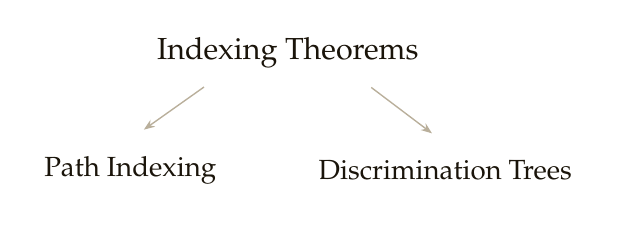
\begin{tikzpicture}[
    root/.style={font=\fontsize{11}{13}\selectfont\mdseries\color{ink}},
    box/.style={font=\selectfont\color{ink}, align=center, inner sep=6pt},
    bullet/.style={font=\fontsize{6.5}{9}\selectfont\color{inkfaint}, align=left},
    arr/.style={-{Stealth[length=4pt]}, color=inkghst, line width=0.5pt, shorten >=6pt, shorten <=6pt},
  ]
    \node[root] (idx) at (4cm, 0) {Indexing Theorems};

    \node[box] (pi) at (2.0cm, -1.5cm) {Path Indexing};
    \node[box] (dt) at (6.0cm, -1.5cm) {Discrimination Trees};

    \draw[arr] ($(idx.south)!0.5!(idx.south west)$) -- (pi.north);
    \draw[arr] ($(idx.south)!0.5!(idx.south east)$) -- (dt.north);

  \end{tikzpicture}
  \end{center}


  \vspace{3cm}
  \quoteblock{%
    Term indexing was used in the early days of automated deduction, but it \\was undocumented or not emphasized in the literature, and the methods are not well known. As a result, it appears that several of the methods were 'reinvented'. 
    The origins of the two indexing methods remain uncertain. The roots of discrimination-tree indexing appear to lie directly in formula manipulation systems, and the roots of path indexing appear to lie in database technology.
  }{%
  ``Experiments with Discrimination-Tree Indexing and Path Indexing''\\
    William McCune, 1990%
  }
\end{frame}

\pathindexingactivetrue
\begin{frame}[label=navpathindexing]{Path Indexing}
  Our mathlib:
  \vspace{0.8em}

  \begin{codeblockml}
    \begin{tabular*}{\linewidth}{@{\extracolsep{\fill}}lll}
      \textbf{Theorem Name} & \textbf{Statement} & \textbf{Prefix Form} \\
      \midrule
      add\_2\_2          & $2 + 2 = 4$     & $=(+(2,\,2),\;4)$ \\
      add\_2\_666        & $2 + 666 = 668$ & $=(+(2,\,666),\;668)$ \\
      add\_3\_5          & $3 + 5 = 8$     & $=(+(3,\,5),\;8)$ \\
      add\_3\_7          & $3 + 7 = 10$    & $=(+(3,\,7),\;10)$ \\
      le\_of\_le\_of\_eq & $a \leq c$      & ${\leq}\;(*,\;*)$ \\
    \end{tabular*}
  \end{codeblockml}

  \only<2>{
  \vspace{0.8em}

  {\fontsize{7}{12}\selectfont Each theorem generates a number of "paths".\\
  Each "path" has the form \code{[symbol, {\color{yellow}arg-position}, symbol, {\color{yellow}arg-position}, ..., symbol]}.\\
  }
  \vspace{0.8em}
  {\fontsize{7}{12}\selectfont 
  For example, \code{add\_3\_7: = (+ (3,\,7),\,10)} has five symbols, so it generates five paths:}
  \vspace{0.4em}

  \begin{codeblockml}
    \begin{tabular*}{\linewidth}{@{\extracolsep{\fill}}ll}
      \textbf{Symbols (add\_3\_7)} & \textbf{Path} \\
      \midrule
      $=$  & $[=]$ \\
      $+$  & $[=,\;{\color{yellow}1},\;+]$ \\
      $3$  & $[=,\;{\color{yellow}1},\;+,\;{\color{yellow}1},\;3]$ \\
      $7$  & $[=,\;{\color{yellow}1},\;+,\;{\color{yellow}2},\;7]$ \\
      $10$ & $[=,\;{\color{yellow}2},\;10]$ \\
    \end{tabular*}
  \end{codeblockml}
  }

\end{frame}

% --- Path Indexing: Step 1 ---
\begin{frame}{}

  \vspace{0cm}

  Per each theorem, per each symbol: compute its path:
  \vspace{0.6em}

  \begin{codeblockml}
    \begin{tabular*}{\linewidth}{@{\extracolsep{\fill}}ll}
      Symbols (add\_3\_7) & Path \\
      \midrule
      $=$  & $[=]$ \\
      $+$  & $[=,\;{\color{yellow}1},\;+]$ \\
      $3$  & $[=,\;{\color{yellow}1},\;+,\;{\color{yellow}1},\;3]$ \\
      $7$  & $[=,\;{\color{yellow}1},\;+,\;{\color{yellow}2},\;7]$ \\
      $10$ & $[=,\;{\color{yellow}2},\;10]$ \\

      \midrule
      Symbols (add\_3\_5) & Path \\
      \midrule
      $=$  & $[=]$ \\
      $+$  & $[=,\;{\color{yellow}1},\;+]$ \\
      $3$  & $[=,\;{\color{yellow}1},\;+,\;{\color{yellow}1},\;3]$ \\
      $5$  & $[=,\;{\color{yellow}1},\;+,\;{\color{yellow}2},\;5]$ \\
      $8$ & $[=,\;{\color{yellow}2},\;8]$ \\

    \end{tabular*}
  \end{codeblockml}

  \vspace{0.6em}

  And put those paths into a new table:
  \vspace{0.6em}

  \begingroup
  \renewcommand{\arraystretch}{1.3}
  \fontsize{6.5}{8.5}\selectfont
  \begin{tabular*}{\linewidth}{l@{\extracolsep{\fill}}c@{\extracolsep{0pt}\quad}c}
    \noalign{\hrule height 0.6pt}
    \textbf{Path} & \textbf{add\_3\_5} & \textbf{add\_3\_7} \\
    \hline
    \code{[=]}                                                           & $\checkmark$ & $\checkmark$ \\
    \code{[=, {\color{yellow}1}, +]}                                     & $\checkmark$ & $\checkmark$ \\
    \code{[=, {\color{yellow}1}, +, {\color{yellow}1}, 3]}               & $\checkmark$ & $\checkmark$ \\
    \code{[=, {\color{yellow}1}, +, {\color{yellow}2}, 5]}               & $\checkmark$ & \\
    \code{[=, {\color{yellow}1}, +, {\color{yellow}2}, 7]}               & & $\checkmark$ \\
    \code{[=, {\color{yellow}2}, 8]}                                     & $\checkmark$ & \\
    \code{[=, {\color{yellow}2}, 10]}                                    & & $\checkmark$ \\
    \noalign{\hrule height 0.6pt}
  \end{tabular*}
  \endgroup

\end{frame}

% --- Path Indexing: Step 2 ---
\begin{frame}{Path Indexing}
  \begingroup
  \renewcommand{\arraystretch}{1.3}
  \fontsize{6.5}{8.5}\selectfont
  \begin{tabular*}{\linewidth}{l@{\extracolsep{\fill}}c@{\extracolsep{0pt}\quad}c}
    \noalign{\hrule height 0.6pt}
    \textbf{Path} & \textbf{add\_3\_5} & \textbf{add\_3\_7} \\
    \hline
    \code{[=]}                                                           & $\checkmark$ & $\checkmark$ \\
    \code{[=, {\color{yellow}1}, +]}                                     & $\checkmark$ & $\checkmark$ \\
    \code{[=, {\color{yellow}1}, +, {\color{yellow}1}, 3]}               & $\checkmark$ & $\checkmark$ \\
    \code{[=, {\color{yellow}1}, +, {\color{yellow}2}, 5]}               & $\checkmark$ & \\
    \code{[=, {\color{yellow}1}, +, {\color{yellow}2}, 7]}               & & $\checkmark$ \\
    \code{[=, {\color{yellow}2}, 8]}                                     & $\checkmark$ & \\
    \code{[=, {\color{yellow}2}, 10]}                                    & & $\checkmark$ \\
    \noalign{\hrule height 0.6pt}
  \end{tabular*}
  \endgroup

  \only<2>{
  \vspace{0.3cm}
  Suppose our goal is \code{3 + 7 = 10}.\\[0.1cm]
  Compute the path of each symbol of our goal, and intersect the theorem sets:
  \setlength{\jot}{0pt}
  \begin{flalign*}
    &\code{[=]} &\;\{{\fontsize{6.5}{8.5}\selectfont\textbf{add\_3\_5}},\;{\fontsize{6.5}{8.5}\selectfont\textbf{add\_3\_7}}\}\\
    &\code{[=, {\color{yellow}1}, +]} &\cap\;\{{\fontsize{6.5}{8.5}\selectfont\textbf{add\_3\_5}},\;{\fontsize{6.5}{8.5}\selectfont\textbf{add\_3\_7}}\}\\
    &\code{[=, {\color{yellow}1}, +, {\color{yellow}1}, 3]} &\cap\;\{{\fontsize{6.5}{8.5}\selectfont\textbf{add\_3\_5}},\;{\fontsize{6.5}{8.5}\selectfont\textbf{add\_3\_7}}\}\\
    &\code{[=, {\color{yellow}1}, +, {\color{yellow}2}, 7]} &\cap\;\{{\fontsize{6.5}{8.5}\selectfont\textbf{add\_3\_7}}\}\\
    &\code{[=, {\color{yellow}2}, 10]} &\cap\;\{{\fontsize{6.5}{8.5}\selectfont\textbf{add\_3\_7}}\}\\[4pt]
    &&=\;\{{\fontsize{6.5}{8.5}\selectfont\textbf{add\_3\_7}}\}
  \end{flalign*}
  }

  \only<2>{We found our theorem candidate: \fontsize{6.5}{8.5}\selectfont\textcolor{green}{\textbf{add\_3\_7}}}.
\end{frame}


\begin{frame}{}
  \begin{center}
  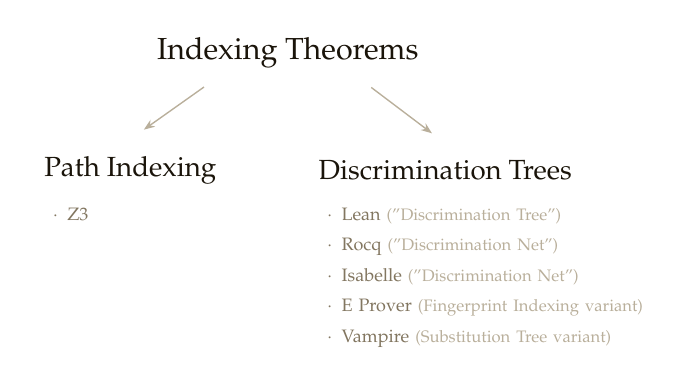
\begin{tikzpicture}[
    root/.style={font=\fontsize{11}{13}\selectfont\mdseries\color{ink}},
    box/.style={font=\selectfont\color{ink}, align=center, inner sep=6pt},
    bullet/.style={font=\fontsize{6.5}{9}\selectfont\color{inkfaint}, align=left},
    arr/.style={-{Stealth[length=4pt]}, color=inkghst, line width=0.5pt, shorten >=6pt, shorten <=6pt},
  ]
    \node[root] (idx) at (4cm, 0) {Indexing Theorems};

    \node[box] (pi) at (2.0cm, -1.5cm) {Path Indexing};
    \node[box] (dt) at (6.0cm, -1.5cm) {Discrimination Trees};

    \draw[arr] ($(idx.south)!0.5!(idx.south west)$) -- (pi.north);
    \draw[arr] ($(idx.south)!0.5!(idx.south east)$) -- (dt.north);

    \node[bullet, anchor=north west, text width=2.5cm, visible on=<2->] at ($(pi.west)+(0.2cm,-0.35cm)$) {%
      $\cdot$\enspace{}Z3\\[2pt]%
    };

    \node[bullet, anchor=north west, text width=4.2cm, visible on=<2->] at ($(dt.west)+(0.2cm,-0.35cm)$) {%
      $\cdot$\enspace{}Lean {\fontsize{6}{7}\selectfont\color{inkghst}("Discrimination Tree")}\\[2pt]%
      $\cdot$\enspace{}Rocq {\fontsize{6}{7}\selectfont\color{inkghst}("Discrimination Net")}\\[2pt]%
      $\cdot$\enspace{}Isabelle {\fontsize{6}{7}\selectfont\color{inkghst}("Discrimination Net")}\\[2pt]%
      $\cdot$\enspace{}E Prover {\fontsize{6}{7}\selectfont\color{inkghst}(Fingerprint Indexing variant)}\\[2pt]%
      $\cdot$\enspace{}Vampire {\fontsize{6}{7}\selectfont\color{inkghst}(Substitution Tree variant)}%
    };
  \end{tikzpicture}
  \end{center}


  \quoteblock{%
    Two different indexing methods are used: discrimination-tree indexing \\and path indexing.
    Some types of term are much better handled by one or the other of the indexing methods. Thus, no clear winner existed between the two methods.

    {\ldots}

    The strongest conclusion from the experiments  is that discrimination indexing is a clear winner over path indexing for generalization retrieval on the types of term with which I experimented.

  }{%
   \vspace{0.2cm}
  ``Experiments with Discrimination-Tree Indexing and Path Indexing''\\
    William McCune, 1990%
  }
\end{frame}

\pathindexingactivefalse
\dtactivate

\dtpart{Trie}
\begin{frame}[label=navtrie]{Discrimination Trees}
  Discrimination tree is a trie

  \only<2->{
  \vspace{0.8em}
  Trie nodes is something we do know\\
  Trie leaves is something we WANT to know
  }

  \only<3->{
  \vspace{0.8em}
  For example,

  \begin{center}
  \scalebox{0.9}{%
  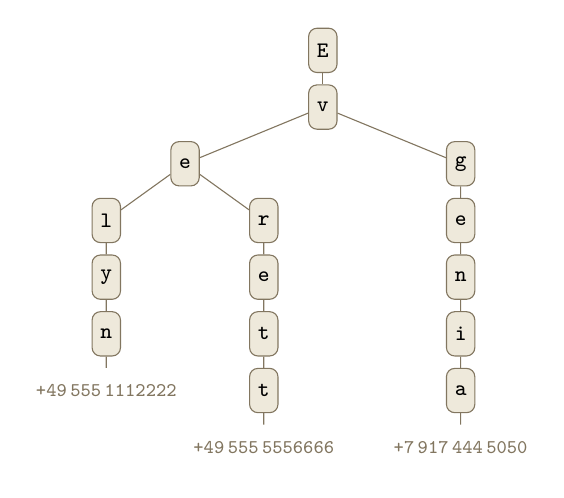
\begin{tikzpicture}[
    every node/.style={draw=inkfaint, rounded corners=3pt, fill=sidebarbg,
      font=\ttfamily\fontsize{8}{10}\selectfont, inner sep=3pt, minimum height=16pt},
    val/.style={draw=none, fill=none, font=\ttfamily\fontsize{7}{8}\selectfont\color{inkfaint}},
    edge from parent/.style={draw=inkfaint},
    level distance=0.72cm,
    level 1/.style={sibling distance=7.0cm},
    level 2/.style={sibling distance=3.5cm},
    level 3/.style={sibling distance=2.0cm},
  ]
  \node {E}
    child { node {v}
      child { node {e}
        child { node {l}
          child { node {y}
            child { node {n}
              child { node[val] {+49\,555\,1112222} }
            }
          }
        }
        child { node {r}
          child { node {e}
            child { node {t}
              child { node {t}
                child { node[val] {+49\,555\,5556666} }
              }
            }
          }
        }
      }
      child { node {g}
        child { node {e}
          child { node {n}
            child { node {i}
              child { node {a}
                child { node[val] {+7\,917\,444\,5050} }
              }
            }
          }
        }
      }
    };
  \end{tikzpicture}}%
  \end{center}
  }
\end{frame}

\begin{frame}{Discrimination Trees}
  Our mathlib:
  \vspace{0.8em}

  \begin{codeblockml}
    \begin{tabular*}{\linewidth}{@{\extracolsep{\fill}}lll}
      \textbf{Theorem Name} & \textbf{Statement} & \textbf{Prefix Form} \\
      \midrule
      add\_2\_2          & $2 + 2 = 4$     & $=(+(2,\,2),\;4)$ \\
      add\_2\_666        & $2 + 666 = 668$ & $=(+(2,\,666),\;668)$ \\
      add\_3\_5          & $3 + 5 = 8$     & $=(+(3,\,5),\;8)$ \\
      add\_3\_7          & $3 + 7 = 10$    & $=(+(3,\,7),\;10)$ \\
      le\_of\_le\_of\_eq & $a \leq c$      & ${\leq}\;(*,\;*)$ \\
    \end{tabular*}
  \end{codeblockml}

  \only<2>{
  \vspace{-0.15cm}
  \begin{center}
  {%
  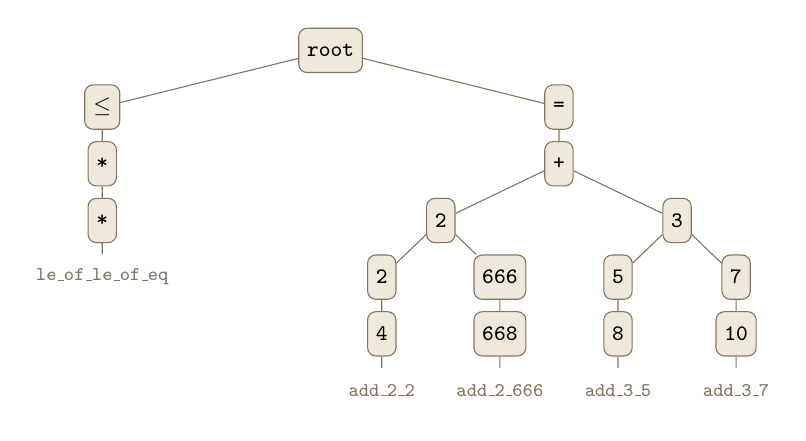
\begin{tikzpicture}[
    every node/.style={draw=inkfaint, rounded corners=3pt, fill=sidebarbg,
      font=\ttfamily\fontsize{8}{10}\selectfont, inner sep=3pt, minimum height=16pt},
    val/.style={draw=none, fill=none, font=\ttfamily\fontsize{7}{8}\selectfont\color{inkfaint}},
    edge from parent/.style={draw=inkfaint},
    level distance=0.72cm,
    level 1/.style={sibling distance=5.8cm},
    level 2/.style={sibling distance=3.5cm},
    level 3/.style={sibling distance=3.0cm},
    level 4/.style={sibling distance=1.5cm},
    level 5/.style={sibling distance=1.5cm},
    level 6/.style={sibling distance=1.5cm},
  ]
  \node {root}
    child { node {$\leq$}
      child { node {*}
        child { node {*}
          child { node[val] {le\_of\_le\_of\_eq} }
        }
      }
    }
    child { node {=}
      child { node {+}
        child { node {2}
          child { node {2}
            child { node {4}
              child { node[val] {add\_2\_2} }
            }
          }
          child { node {666}
            child { node {668}
              child { node[val] {add\_2\_666} }
            }
          }
        }
        child { node {3}
          child { node {5}
            child { node {8}
              child { node[val] {add\_3\_5} }
            }
          }
          child { node {7}
            child { node {10}
              child { node[val] {add\_3\_7} }
            }
          }
        }
      }
    };
  \end{tikzpicture}}%
  \end{center}
  }
\end{frame}



\begin{frame}{Discrimination Trees}
  \vspace{-0.35cm}
  \begin{center}
  {%
  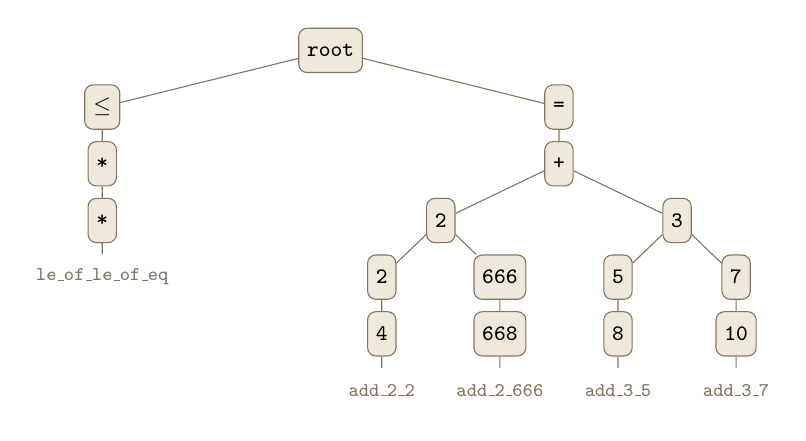
\begin{tikzpicture}[
    every node/.style={draw=inkfaint, rounded corners=3pt, fill=sidebarbg,
      font=\ttfamily\fontsize{8}{10}\selectfont, inner sep=3pt, minimum height=16pt},
    val/.style={draw=none, fill=none, font=\ttfamily\fontsize{7}{8}\selectfont\color{inkfaint}},
    edge from parent/.style={draw=inkfaint},
    level distance=0.72cm,
    level 1/.style={sibling distance=5.8cm},
    level 2/.style={sibling distance=3.5cm},
    level 3/.style={sibling distance=3.0cm},
    level 4/.style={sibling distance=1.5cm},
    level 5/.style={sibling distance=1.5cm},
    level 6/.style={sibling distance=1.5cm},
  ]
  \node {root}
    child { node {$\leq$}
      child { node {*}
        child { node {*}
          child { node[val] {le\_of\_le\_of\_eq} }
        }
      }
    }
    child { node {=}
      child { node {+}
        child { node {2}
          child { node {2}
            child { node {4}
              child { node[val] {add\_2\_2} }
            }
          }
          child { node {666}
            child { node {668}
              child { node[val] {add\_2\_666} }
            }
          }
        }
        child { node {3}
          child { node {5}
            child { node {8}
              child { node[val] {add\_3\_5} }
            }
          }
          child { node {7}
            child { node {10}
              child { node[val] {add\_3\_7} }
            }
          }
        }
      }
    };
  \end{tikzpicture}}%
  \end{center}

  This is our discrimination tree, aka \code{DiscrTree}.\\[1em]

  Lean and Mathlib maintain around 15 different \code{DiscrTree}s. Nodes always contain Lean expressions, leaves contain different stuff.\\[1em]

  \code{DiscrTree $\alpha$}: nodes are expressions, each leaf is \code{$\alpha$}.\\
  \code{DiscrTree Name}: nodes are expressions, each leaf is a \code{Name}\\
  \code{DiscrTree SimpTheorem}: nodes are expressions, each leaf is a \code{SimpTheorem}\\[1em]

\end{frame}


\dtpart{Lean and Mathlib}
\begin{frame}[label=navleanmathlib]{Discrimination Trees: Lean and Mathlib}
  \vspace{-0.1cm}
  \renewcommand{\arraystretch}{1.4}
  \begin{tabular}{@{}m{2cm}m{2.7cm}m{4cm}@{}}
    \textbf{Used By} & \textbf{Attribute} & \textbf{Storage} \\
    \toprule
    {\fontsize{7}{8.5}\selectfont{typeclass instances}} & \code{@[instance]} & \code{DiscrTree InstanceEntry} \\
    {\fontsize{7}{8.5}\selectfont{unification hints}} & \code{@[unification\_hint]} & \code{DiscrTree Name} \\
    \code{simp} {\fontsize{7}{8.5}\selectfont{(theorems)}} & \code{@[simp]} & \code{DiscrTree SimpTheorem} \\
    \code{simp} {\fontsize{7}{8.5}\selectfont{(simprocs)}} & \code{@[simproc]} & \code{DiscrTree SimprocEntry} \\
    \code{rfl} & \code{@[refl]} & \code{DiscrTree Name} \\
    \code{symm} & \code{@[symm]} & \code{DiscrTree Name} \\
    \code{ext} & \code{@[ext]} & \code{DiscrTree ExtTheorem} \\
    \code{norm\_num} & \code{@[norm\_num]} & \code{DiscrTree NormNumExt} \\
    \code{positivity} & \code{@[positivity]} & \code{DiscrTree PositivityExt} \\
    \code{push} & \code{@[push]} & \code{DiscrTree SimpTheorem} \\
    \code{pull} & \code{@[push]} & \code{DiscrTree PullTheorem} \\
    \code{fun\_prop} & \code{@[fun\_prop]} & \code{RefinedDiscrTree GeneralTheorem} \\
    \code{exact?} / \code{apply?} & {\color{inkfaint} {\fontsize{7}{8.5}\selectfont{all imported declarations}}} & \code{LazyDiscrTree (Name $\times$ DeclMod)} \\
    \code{rw?} & {\color{inkfaint} {\fontsize{7}{8.5}\selectfont{all imported declarations}}} & \code{LazyDiscrTree (Name $\times$ RwDirection)} \\
    \code{rw??} & {\color{inkfaint} {\fontsize{7}{8.5}\selectfont{all imported declarations}}} & \code{RefinedDiscrTree RewriteLemma} \\[0.4em]
    \bottomrule
  \end{tabular}

\end{frame}

\begin{frame}{Discrimination Trees: Lean and Mathlib}
  \vspace{-0.1cm}
  \renewcommand{\arraystretch}{1.4}
  \begin{tabular}{@{}m{2cm}m{2.7cm}m{4cm}@{}}
    \textbf{Used By} & \textbf{Attribute} & \textbf{Storage} \\
    \toprule
    {\fontsize{7}{8.5}\selectfont{typeclass instances}} & \code{@[instance]} & \code{DiscrTree InstanceEntry} \\
    {\fontsize{7}{8.5}\selectfont{unification hints}} & \code{@[unification\_hint]} & \code{DiscrTree Name} \\
    \code{simp} {\fontsize{7}{8.5}\selectfont{(theorems)}} & \code{@[simp]} & \code{DiscrTree SimpTheorem} \\
    \multicolumn{3}{@{}c}{{\color{inkfaint}\fontsize{7}{8.5}\selectfont $\cdots$}} \\[0.2em]
    \code{exact?} / \code{apply?} & {\color{inkfaint} {\fontsize{7}{8.5}\selectfont{all imported declarations}}} & \code{LazyDiscrTree (Name $\times$ DeclMod)} \\
    \code{rw??} & {\color{inkfaint} {\fontsize{7}{8.5}\selectfont{all imported declarations}}} & \code{RefinedDiscrTree RewriteLemma} \\[0.4em]
    \bottomrule
  \end{tabular}

  \vspace{0.2cm}
  \quoteblock{%
    During the compilation of Mathlib, Lean spends approximately 14\% of its time running the discrimination trees that allow for efficient association of terms with values.%
  }{%
    ``Growing Mathlib: maintenance of a large scale mathematical library''\\
    Baanen, Ballard, Commelin, Chen, Rothgang, Testa, 2025%
  }

  \only<2->{
  \vspace{0.2cm}
  A single large discrimination tree?
  \only<3->{
    \vspace{0.1cm}
    \begin{itemize}
      \item[{\visible<4->{\raise2pt\hbox{\fontsize{4}{4}\selectfont\textcolor{inkghst}{$\blacktriangleright$}}}}] \visible<4->{Leaves store different stuff (e.g. \code{InstanceEntry} vs \code{Name}) - not a problem}
      \item[{\visible<5->{\raise2pt\hbox{\fontsize{4}{4}\selectfont\textcolor{inkghst}{$\blacktriangleright$}}}}] \visible<5->{Different theorems are processed (e.g. \code{@[simp]} vs \code{@[norm\_num]}) - not a problem}
      \item[{\visible<6->{\raise2pt\hbox{\fontsize{4}{4}\selectfont\textcolor{inkghst}{$\blacktriangleright$}}}}] \visible<6->{Actual reason: \textbf{nodes} store different stuff (e.g. \code{exact?} full expression, \code{simp} LHS)}
    \end{itemize}
    }
  }
\end{frame}


\dtdeactivate
\indexingsubsecfalse


\subsection{Example}

\begin{frame}{Global Search: Example}

  Our Mathlib:

  \vspace{0.3cm}

  \begin{codeblockml}
  \begin{tabular}{@{}l@{~}l@{}}
  theorem Nat.add\_comm & : {\color{inkfaint}$\forall$ (n m : Nat), n + m = m + n} \\[0.5em]
  theorem Nat.zero\_le  & : {\color{inkfaint}$\forall$ (n : Nat), 0 $\le$ n} \\[0.5em]
  theorem Nat.le\_refl  & : {\color{inkfaint}$\forall$ (n : Nat), n $\le$ n} \\[0.5em]
  theorem Nat.le\_succ  & : {\color{inkfaint}$\forall$ (n : Nat), n $\le$ n.succ}
  \end{tabular}
  \end{codeblockml}

  \vspace{0.5cm}

  Our goal:

  \vspace{0.25cm}

  \begin{codeblockml}
    {$\vdash$} {\color{inkfaint} 0 {$\le$} 5}
  \end{codeblockml}

  \vspace{0.5cm}

  We call \code{exact?}, and the global search among all Mathlib lemmas starts:

  \vspace{0.2cm}

  \begin{itemize}
    \item We convert each Mathlib theorem into \code{[Key, Key, Key]}, 
    \\ and put all theorems into a \textbf{DiscrTree}
    \item We convert our goal into \code{[Key, Key, Key]}
    \item We match the resulting \textbf{DiscrTree} to our goal!
  \end{itemize}

\end{frame}

\begin{frame}{Global Search: What We Do To Mathlib}
  \vspace{-6px}
  \begin{codeblockml}
  theorem Nat.add\_comm : {\color{inkfaint}$\forall$ (n m : Nat), n + m = m + n}

  \only<2->{
  \vspace{0.7px}
  theorem Nat.add\_comm : {\color{inkghst}$\forall$ (n m : Nat), }{\color{inkfaint}Eq Nat (Nat.add n m) (Nat.add m n)}
  }

  \only<3->{
  \vspace{0.7px}
  theorem Nat.add\_comm : {\color{inkfaint}.mkAppN (.const `Eq) \#[.const `Nat, .mkAppN (.const `Nat.add) \#[.fvar `n, .fvar `m], .mkAppN (.const `Nat.add) \#[.fvar `m, .fvar `n]]}%
  }
  \end{codeblockml}

  \only<3->{
  \begin{columns}[T, onlytextwidth]
    \begin{column}{0.45\textwidth}
      \begin{codeblockml}
        \code{inductive Expr}\\[0.3em]
        {\fontsize{6}{8.5}\selectfont\ttfamily
        \hspace*{0.7em}| bvar\ \ \ \ : Nat\\
        \hspace*{0.7em}| fvar\ \ \ \ : FVarId\\
        \hspace*{0.7em}| mvar\ \ \ \ : MVarId\\
        \hspace*{0.7em}| sort\ \ \ \ : Level\\
        \hspace*{0.7em}| const\ \ \ : Name → List Level\\
        \hspace*{0.7em}| app\ \ \ \ \ : Expr → Expr\\
        \hspace*{0.7em}| lam\ \ \ \ \ : Name → Expr → Expr\\
        \hspace*{0.7em}| forallE : \ Name → Expr → Expr\\
        \hspace*{0.7em}| letE\ \ \ \ : \ Name → ...\\
        \hspace*{0.7em}| lit\ \ \ \ \ : Literal\\
        \hspace*{0.7em}| mdata\ \ \ : MData → Expr\\
        \hspace*{0.7em}| proj\ \ \ \ : Name → Nat → Expr\\
        }%
      \end{codeblockml}
    \end{column}
    \begin{column}{0.54\textwidth}
      \only<4->{
      \begin{tikzpicture}[
        every node/.style={
          draw=inkfaint, rounded corners=2pt, fill=sidebarbg,
          font=\ttfamily\fontsize{6}{8.5}\selectfont,
          inner xsep=3pt, inner ysep=3pt, align=center
        }
      ]
      \node (mn1)  at (2.5,  0)      {\only<4>{.mkAppN}\only<5->{\sout{.mkAppN}}};
      \node (eq)   at (0.5,  -1.05)  {.const\\`Eq};
      \node (nat1) at (1.8, -1.05)  {.const\\`Nat};
      \node (mn2)  at (3.1,  -0.95)  {\only<4>{.mkAppN}\only<5->{\sout{.mkAppN}}};
      \node (mn3)  at (4.5,  -0.95)  {\only<4>{.mkAppN}\only<5->{\sout{.mkAppN}}};
      \node (add1) at (0.5,  -2.2)   {.const\\`Nat.add};
      \node (n1)   at (1.49,  -2.2)   {.fvar \\`n};
      \node (m1)   at (2.32,  -2.2)   {.fvar \\`m};
      \node (add2) at (3.4, -2.2)   {.const\\`Nat.add};
      \node (m2)   at (4.39,  -2.2)   {.fvar \\`m};
      \node (n2)   at (5.2,  -2.2)   {.fvar \\`n};
      \draw[color=inkfaint] (mn1)--(eq);
      \draw[color=inkfaint] (mn1)--(nat1);
      \draw[color=inkfaint] (mn1)--(mn2);
      \draw[color=inkfaint] (mn1)--(mn3);
      \draw[color=inkfaint] (mn2)--(add1);
      \draw[color=inkfaint] (mn2)--(n1);
      \draw[color=inkfaint] (mn2)--(m1);
      \draw[color=inkfaint] (mn3)--(add2);
      \draw[color=inkfaint] (mn3)--(m2);
      \draw[color=inkfaint] (mn3)--(n2);
      \end{tikzpicture}
      }
    \end{column}
  \end{columns}
  }

  \only<5->{
    \vspace{5px}
    \begin{codeblockml}
    theorem Nat.add\_comm : {\color{inkfaint} [.const `Eq 3, .const `Nat 0, .const `Nat.add 2, .fvar `n 0, .fvar `m 0, .const `Nat.add 2, .fvar `m 0, .fvar `n 0]
    }
    \end{codeblockml}
  }
\end{frame}


\begin{frame}{Global Search: What We Do To Mathlib}

  \begin{codeblockml}
  theorem Nat.add\_comm : {\color{inkfaint} [Expr.const `Eq 3, Expr.const `Nat 0, Expr.const `Nat.add 2, Expr.fvar `n 0, Expr.fvar `m 0, Expr.const `Nat.add 2, Expr.fvar `m 0, Expr.fvar `n 0]
  }
  \end{codeblockml}

  \begin{center}
  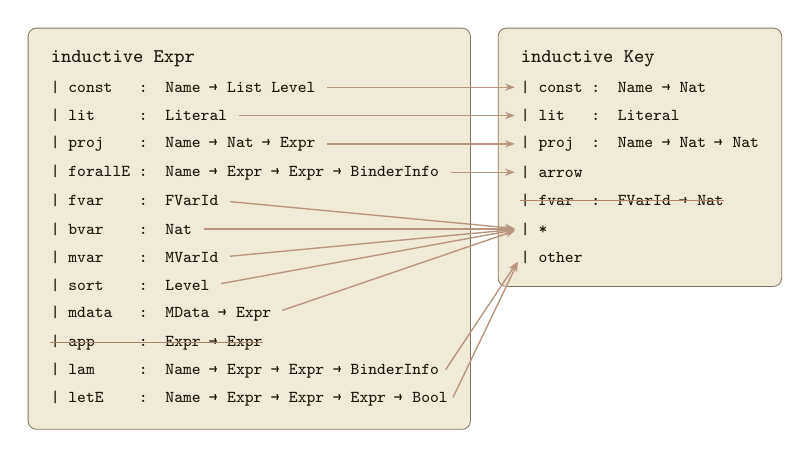
\begin{tikzpicture}[
    row/.style    = {font=\fontsize{6}{8.5}\selectfont\ttfamily\color{ink}, anchor=west, inner sep=0pt},
    hdr/.style    = {font=\fontsize{7}{9}\selectfont\ttfamily\bfseries\color{ink}, anchor=west, inner sep=0pt},
    box/.style    = {fill=codebg, rounded corners=3pt, draw=inkfaint, line width=0.3pt, inner sep=8pt},
    arr/.style    = {-{Stealth[length=3.5pt]}, color=keyterra!60, line width=0.5pt, shorten <=4pt, shorten >=2pt},  
    arrstar/.style= {-{Stealth[length=3.5pt]}, color=keyterra!60, line width=0.5pt, shorten <=4pt, shorten >=2pt},
  ]
    \def\lx{0cm}
    \def\rx{5.97cm}
    \def\rs{0.36cm}  % row spacing

    % ── Expr column ──
    \node[hdr] (eh)  at (\lx, 0)           {inductive Expr};
    \node[row] (eco) at (\lx, -1*\rs)      {| const\ \ \ : Name → List Level};
    \node[row] (eli) at (\lx, -2*\rs)      {| lit\ \ \ \ \ : Literal};
    \node[row] (epr) at (\lx, -3*\rs)      {| proj\ \ \ \ : Name → Nat → Expr};
    \node[row] (efa) at (\lx, -4*\rs)      {| forallE : \ Name → Expr → Expr → BinderInfo};
    \node[row] (efv) at (\lx, -5*\rs)      {| fvar\ \ \ \ : FVarId};
    \node[row] (ebv) at (\lx, -6*\rs)      {| bvar\ \ \ \ : Nat};
    \node[row] (emv) at (\lx, -7*\rs)      {| mvar\ \ \ \ : MVarId};
    \node[row] (eso) at (\lx, -8*\rs)      {| sort\ \ \ \ : Level};
    \node[row] (emd) at (\lx, -9*\rs)      {| mdata\ \ \ : MData → Expr};
    \node[row] (eap) at (\lx, -10*\rs)     {| app\ \ \ \ \ : Expr → Expr};
    \node[row] (ela) at (\lx, -11*\rs)     {| lam\ \ \ \ \ : Name → Expr → Expr → BinderInfo};
    \node[row] (ele) at (\lx, -12*\rs)     {| letE\ \ \ \ : \ Name → Expr → Expr → Expr → Bool };

    \begin{scope}[on background layer]
      \node[box, fit=(eh)(eco)(efv)(eli)(epr)(ebv)(emv)(eso)(emd)(eap)(ela)(ele)(efa)] {};
    \end{scope}

    % ── Key column ──
    \node[hdr] (kh)  at (\rx, 0)           {inductive Key};
    \node[row] (kco) at (\rx, -1*\rs)      {| const : Name → Nat};
    \node[row] (kli) at (\rx, -2*\rs)      {| lit\ \ \ : Literal};
    \node[row] (kpr) at (\rx, -3*\rs)      {| proj\ \ : Name → Nat → Nat};
    \node[row] (kar) at (\rx, -4*\rs)      {| arrow};
    \node[row] (kfv) at (\rx, -5*\rs)      {| fvar\ \ : FVarId → Nat};
    \node[row] (kst) at (\rx, -6*\rs)      {| *};
    \node[row] (kot) at (\rx, -7*\rs)      {| other};

    \begin{scope}[on background layer]
      \node[box, fit=(kh)(kco)(kfv)(kli)(kpr)(kst)(kot)(kar)] {};
    \end{scope}

    % ── Arrows (direct matches) ──
    \draw[arr] (eco.east) -- (kco.west);
    \draw[arr] (eli.east) -- (kli.west);
    \draw[arr] (epr.east) -- (kpr.west);
    \draw[arr] (efa.east) -- (kar.west);
    % ── Star arrows ──
    \draw[arr] (efv.east) -- (kst.west);
    \draw[arr] (ebv.east) -- (kst.west);
    \draw[arr] (emv.east) -- (kst.west);
    \draw[arr] (eso.east) -- (kst.west);
    \draw[arr] (emd.east) -- (kst.west);
    \draw[color=keyterra!70, line width=0.5pt] (eap.west) -- (eap.east);
    \draw[color=keyterra!70, line width=0.5pt] (kfv.west) -- (kfv.east);
    \draw[arr] ([yshift=-3pt]ela.east) -- (kot.west);
    \draw[arr] ([yshift=-3pt]ele.east) -- (kot.west);


  \end{tikzpicture}
  \end{center}


  \begin{codeblockml}
  theorem Nat.add\_comm : {\color{inkfaint} [Key.const `Eq 3, Key.const `Nat 0, Key.const `Nat.add 2, *, *, Key.const `Nat.add 2, *, *]
  }
  \end{codeblockml}

\end{frame}



\begin{frame}{Global Search: What We Do To Mathlib}

  \vspace{-0.2cm}
  \textbf{BEFORE:}
  \vspace{0.2cm}

  \begin{codeblockml}
    theorem Nat.add\_comm : {\color{inkfaint}{\color{inkfaint}$\forall$ (n m : Nat), n + m = m + n}}
  \end{codeblockml}

  \vspace{0.2cm}

  \textbf{STEPS:}

  \vspace{0.2cm}

  \begin{codeblockml}
  \textcolor{keyterra}{1. We have a Mathlib theorem}
  \vspace{0.1cm}


  \hspace{0.35cm}
  theorem Nat.add\_comm (n m : Nat) : {\color{inkfaint}n + m = m + n}

  \vspace{0.1cm}
  \textcolor{keyterra}{2. Reduce the expression, strip foralls}
  \vspace{0.1cm}

  \hspace{0.35cm}
  theorem Nat.add\_comm : {\color{inkghst}$\forall$ (n m : Nat), }{\color{inkfaint}Eq Nat (Nat.add n m) (Nat.add m n)}

  \vspace{0.1cm}
  \textcolor{keyterra}{3. Turn Expr tree into a list of Exprs}
  \vspace{0.1cm}

  \hspace{0.35cm}
  theorem Nat.add\_comm : {\color{inkfaint} [Expr.const `Eq 3,
  Expr.const `Nat 0,  Expr.const 
  
  \hspace{0.35cm}
  `Nat.add 2, Expr.fvar `n 0, Expr.fvar `m 0,
  Expr.const `Nat.add 2,
  
  \hspace{0.37cm}
  Expr.fvar `m 0, Expr.fvar `n 0]
  }

  \vspace{0.1cm}
  \textcolor{keyterra}{4. Map a list of Exprs to a list of Keys}
  \vspace{0.1cm}

  \hspace{0.35cm}
  theorem Nat.add\_comm : {\color{inkfaint} [Key.const `Eq 3,
  Key.const `Nat 0,

  \hspace{0.36cm}
  Key.const `Nat.add 2, *, *,
  Key.const `Nat.add 2, *, *
  ]}
  \end{codeblockml}


  \vspace{0.2cm}
  \textbf{AFTER:}
  \vspace{0.2cm}

  \begin{codeblockml}
      theorem Nat.add\_comm : {\color{inkfaint} [Key.const `Eq 3,
  Key.const `Nat 0,
  Key.const `Nat.add 2,
  *, *,
  Key.const `Nat.add 2, *, *
  ]}
  \end{codeblockml}

\end{frame}




\begin{frame}{Global Search: What We Do To Our Goal}

  \vspace{-0.2cm}
  \textbf{BEFORE:}
  \vspace{0.2cm}

  \begin{codeblockml}
    {$\vdash$}  \color{inkfaint}{0 $\le$ 5}
  \end{codeblockml}


  \vspace{0.6cm}

  \textbf{STEPS:}

  \vspace{0.2cm}

  \begin{codeblockml}
  \textcolor{keyterra}{1. We have a goal}
  \vspace{0.1cm}

  \hspace{0.35cm}
  {$\vdash$} {\color{inkfaint} 0 $\le$ 5}

  \vspace{0.1cm}
  \textcolor{keyterra}{2. Reduce the expression, strips foralls}
  \vspace{0.1cm}

  \hspace{0.35cm}
  {$\vdash$} {\color{inkfaint} Nat.le 0 5}

  \vspace{0.1cm}
  \textcolor{keyterra}{3. Turn Expr tree into a list of Exprs}
  \vspace{0.1cm}

  \hspace{0.35cm}
  {$\vdash$} {\color{inkfaint} [Expr.const `Nat.le 2, Expr.lit 0, Expr.lit 5]}

  \vspace{0.1cm}
  \textcolor{keyterra}{4. Map a list of Exprs to a list of Keys}
  \vspace{0.1cm}

  \hspace{0.35cm}
  {$\vdash$} {\color{inkfaint} [Key.const `Nat.le 2, Key.lit 0, Key.lit 5]}
  \end{codeblockml}


  \vspace{0.6cm}

  \textbf{AFTER:}
  
  \vspace{0.2cm}

  \begin{codeblockml}
  {$\vdash$} \color{inkfaint}{[Key.const `Nat.le 2, Key.lit 0, Key.lit 5]}
  \end{codeblockml}

\end{frame}


\begin{frame}{Global search: DiscrTree}
  All Mathlib lemmas:

  \vspace{0.5cm}
  \begin{codeblockml}
  \begin{tabular}{@{}l@{~}l@{}}
  theorem Nat.add\_comm & \parbox[t]{7.5cm}{: {\color{inkfaint}[Key.const `Eq 3, Key.const `Nat 0, Key.const `Nat.add 2,\\\phantom{: [}
  *, *, Key.const `Nat.add 2, *, *]}} \\[1.6em]
  theorem Nat.zero\_le  & : {\color{inkfaint}[Key.const `Nat.le 2, Key.lit 0, *]} \\[0.5em]
  theorem Nat.le\_refl  & : {\color{inkfaint}[Key.const `Nat.le 2, *, *]} \\[0.5em]
  theorem Nat.le\_succ  & : {\color{inkfaint}[Key.const `Nat.le 2, *, *]}
  \end{tabular}
  \end{codeblockml}
  \vspace{2.85cm}

  Our goal:

  \vspace{0.2cm}
  \begin{codeblockml}
    {$\vdash$} {\color{inkfaint}
      [Key.const `Nat.le 2, Key.lit 0, Key.lit 5]
      }
  \end{codeblockml}
\end{frame}

\begin{frame}{Global Search: DiscrTree}

  \vspace{-0.3cm}

  \begin{codeblockml}
  \begin{tabular}{@{}l@{~}l@{}}
  theorem Nat.add\_comm & \alt<2->{\parbox[t]{7.5cm}{: {\color{inkfaint}[Key.const `Eq 3, Key.const `Nat 0, Key.const `Nat.add 2,\\\phantom{: [}
   *, *, Key.const `Nat.add 2, *, *]}}}{: } \alt<2->{\\[1.6em]}{\\[0.5em]}
  theorem Nat.zero\_le  & \alt<3->{: {\color{inkfaint}[Key.const `Nat.le 2, Key.lit 0, *]}}{:} \\[0.5em]
  theorem Nat.le\_refl  & \alt<4->{: {\color{inkfaint}[Key.const `Nat.le 2, *, *]}}{:} \\[0.5em]
  theorem Nat.le\_succ  & \alt<5->{: {\color{inkfaint}[Key.const `Nat.le 2, *, *]}}{:}
  \end{tabular}
  \end{codeblockml}

  \only<2->{
  % \vspace{0.4cm}
  \begin{center}
  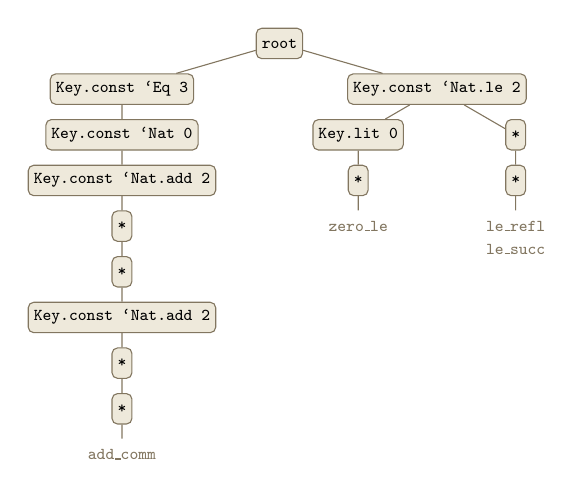
\begin{tikzpicture}[
        every node/.style={draw=inkfaint, rounded corners=2pt, fill=sidebarbg,
          font=\ttfamily\fontsize{6}{7}\selectfont, inner sep=2pt, minimum height=11pt},
        val/.style={draw=none, fill=none,
          font=\ttfamily\fontsize{6}{7}\selectfont\color{inkfaint}},
        edge from parent/.style={draw=inkfaint},
        level distance=0.58cm,
        level 1/.style={sibling distance=4.0cm},
        level 2/.style={sibling distance=2.0cm},
        level 3/.style={sibling distance=1.0cm},
        level 4/.style={sibling distance=1.0cm},
        level 5/.style={sibling distance=1.0cm},
        level 6/.style={sibling distance=1.0cm},
        level 7/.style={sibling distance=1.0cm},
        level 8/.style={sibling distance=1.0cm},
      ]
      \node {root}
        child {
          node[visible on=<2->] {Key.const `Eq 3}
          edge from parent[visible on=<2->]
          child {
            node[visible on=<2->] {Key.const `Nat 0}
            edge from parent[visible on=<2->]
            child {
              node[visible on=<2->] {Key.const `Nat.add 2}
              edge from parent[visible on=<2->]
              child {
                node[visible on=<2->] {*}
                edge from parent[visible on=<2->]
                child {
                  node[visible on=<2->] {*}
                  edge from parent[visible on=<2->]
                  child {
                    node[visible on=<2->] {Key.const `Nat.add 2}
                    edge from parent[visible on=<2->]
                    child {
                      node[visible on=<2->] {*}
                      edge from parent[visible on=<2->]
                      child {
                        node[visible on=<2->] {*}
                        edge from parent[visible on=<2->]
                        child {
                          node[val, visible on=<2->] {add\_comm}
                          edge from parent[visible on=<2->]
                        }
                      }
                    }
                  }
                }
              }
            }
          }
        }
        child {
          node[visible on=<3->] {Key.const `Nat.le 2}
          edge from parent[visible on=<3->]
          child {
            node[visible on=<3->] {Key.lit 0}
            edge from parent[visible on=<3->]
            child {
              node[visible on=<3->] {*}
              edge from parent[visible on=<3->]
              child {
                node[val, visible on=<3->] {zero\_le}
                edge from parent[visible on=<3->]
              }
            }
          }
          child {
            node[visible on=<4->] {*}
            edge from parent[visible on=<4->]
            child {
              node[visible on=<4->] {*}
              edge from parent[visible on=<4->]
              child {
                node[val, visible on=<4->] (mleref) {le\_refl}
                edge from parent[visible on=<4->]
              }
            }
          }
        }
      ;
      \node[val, visible on=<5->, below=-3pt of mleref] {le\_succ};
  \end{tikzpicture}
  \end{center}
  }

\end{frame}




\begin{frame}[<6>]{Global Search: Mathlib + Our Goal}

  All Mathlib lemmas:

  \only<1>{
    \vspace{0.5cm}
    \begin{codeblockml}
    \begin{tabular}{@{}l@{~}l@{}}
    theorem Nat.add\_comm & \parbox[t]{7.5cm}{: {\color{inkfaint}[Key.const `Eq 3, Key.const `Nat 0, Key.const `Nat.add 2,\\\phantom{: [}
    *, *, Key.const `Nat.add 2, *, *]}} \\[1.6em]
    theorem Nat.zero\_le  & : {\color{inkfaint}[Key.const `Nat.le 2, Key.lit 0, *]} \\[0.5em]
    theorem Nat.le\_refl  & : {\color{inkfaint}[Key.const `Nat.le 2, *, *]} \\[0.5em]
    theorem Nat.le\_succ  & : {\color{inkfaint}[Key.const `Nat.le 2, *, *]}
    \end{tabular}
    \end{codeblockml}
    \vspace{2.85cm}
  }

  \only<2->{
  \begin{center}
  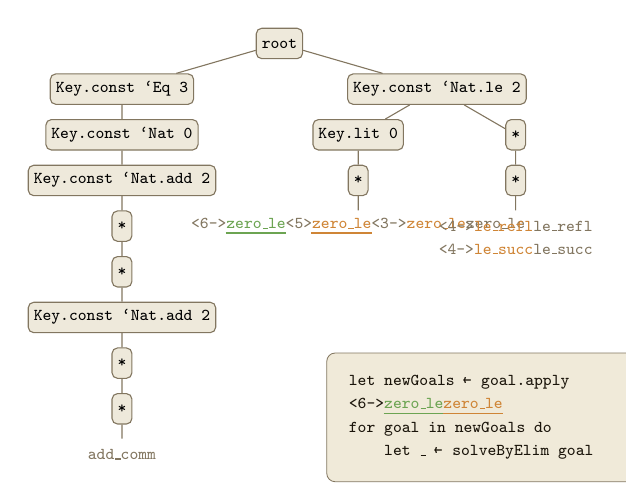
\begin{tikzpicture}[
        every node/.style={draw=inkfaint, rounded corners=2pt, fill=sidebarbg,
          font=\ttfamily\fontsize{6}{7}\selectfont, inner sep=2pt, minimum height=11pt},
        val/.style={draw=none, fill=none,
          font=\ttfamily\fontsize{6}{7}\selectfont\color{inkfaint}},
        edge from parent/.style={draw=inkfaint},
        level distance=0.58cm,
        level 1/.style={sibling distance=4.0cm},
        level 2/.style={sibling distance=2.0cm},
        level 3/.style={sibling distance=1.0cm},
        level 4/.style={sibling distance=1.0cm},
        level 5/.style={sibling distance=1.0cm},
        level 6/.style={sibling distance=1.0cm},
        level 7/.style={sibling distance=1.0cm},
        level 8/.style={sibling distance=1.0cm},
      ]
      \node {root}
        child {
          node {Key.const `Eq 3}
          child {
            node {Key.const `Nat 0}
            child {
              node {Key.const `Nat.add 2}
              child {
                node {*}
                child {
                  node {*}
                  child {
                    node {Key.const `Nat.add 2}
                    child {
                      node {*}
                      child {
                        node {*}
                        child {
                          node[val] {add\_comm}
                        }
                      }
                    }
                  }
                }
              }
            }
          }
        }
        child {
          node {Key.const `Nat.le 2}
          child {
            node {Key.lit 0}
            child {
              node {*}
              child {
                node[val] (nzerole) {
                  \alt<6->{\textcolor{green}{\uline{zero\_le}}}{\alt<5>{\textcolor{yellow}{\uline{zero\_le}}}{\alt<3->{\textcolor{yellow}{zero\_le}}{zero\_le}}}
                }
              }
            }
          }
          child {
            node {*}
            child {
              node {*}
              child {
                node[val] (nleref) {
                  \alt<4->{\textcolor{yellow}{le\_refl}}{le\_refl}
                }
              }
            }
          }
        }
      ;
      \node[val, below=-3pt of nleref] (nlesucc) {
        \alt<4->{\textcolor{yellow}{le\_succ}}{le\_succ}
      };
      \only<5->{
        \node[val, overlay, below=40pt of nzerole, xshift=50pt,
              fill=codebg, rounded corners=3pt, inner sep=8pt, draw=inkfaint, line width=0.3pt,
              font=\ttfamily\fontsize{6}{8.5}\selectfont\color{ink}] {
          \begin{minipage}{3.75cm}
          {let newGoals ← goal.apply \alt<6->{\textcolor{green}{\uline{zero\_le}}}{\textcolor{yellow}{\uline{zero\_le}}}}\\
          for goal in newGoals do\\
          \hspace*{2em}let \_ ← solveByElim goal
          \end{minipage}
        };
      }
      
  \end{tikzpicture}
  \end{center}
  }

  Our goal:

  \vspace{0.2cm}
  \begin{codeblockml}
    {$\vdash$} {\color{inkfaint}
      [Key.const `Nat.le 2, Key.lit 0, Key.lit 5]
      }
  \end{codeblockml}

\end{frame}

\section{Overview}

\begin{frame}{Overview}

  \begin{codeblockml}
    \fontsize{7}{10}\selectfont\raggedright
    example (l$_1$ l$_2$ l$_3$ : List Nat) (h$_1$ : l$_1$.length $\leq$ l$_2$.length) (h$_2$ : l$_3$ = l$_2$) : l$_1$.length $\leq$ l$_3$.length := by\\[0.1cm]
    \hspace*{2em}exact?%
  \end{codeblockml}

  \vspace{0.1cm}

  \begin{codeblockml}
    \fontsize{7}{10}\selectfont\raggedright
    example (l$_1$ l$_2$ l$_3$ : List Nat) (h$_1$ : l$_1$.length $\leq$ l$_2$.length) (h$_2$ : l$_3$ = l$_2$) : l$_1$.length $\leq$ l$_3$.length := by\\[0.1cm]
    \hspace*{2em}exact le\_of\_le\_of\_eq h$_1$ (congrArg List.length (id (Eq.symm h$_2$)))
  \end{codeblockml}


  \vspace{0.3cm}

  
  \makebox[\linewidth][l]{\hspace{-0.09cm}\exactblock{0}}


  \vspace{1.3cm}
  \only<2>{
    \centering{\Large Demo: Real Project}
  }
\end{frame}

\section{Related Tactics}

\begin{frame}{Related Tactics}
\end{frame}


\subsection{Apply?}
\begin{frame}{Related Tactics: Apply?}

  \code{apply?} and \code{exact?} call the same function (\textit{/Lean/Elab/Tactic/LibrarySearch.lean})

  \vspace{0.1cm}

  \begin{itemize}
    \item \code{exact?} calls \code{exact? ref config required requireClose := True}
    \item \code{apply?} calls \code{exact? ref config required requireClose := False}
  \end{itemize}
  
  \vspace{0.3cm}

  \begin{codeblockml}
    {let newGoals ← goal.apply \textcolor{yellow}{\uline{lemma that matched our goal in DiscrTree}}}\\
    \textcolor{inkfaint}{\hspace{0em}{-}{-} lemma is guaranteed to be returned whatever happens to the remaining subgoals}
    \\
    for goal in newGoals do\\
    \hspace*{2em}let \_ ← solveByElim goal
  \end{codeblockml}
\end{frame}

\subsection{Rw?}
\begin{frame}{Related Tactics: Rw?}

  {\setlength{\leftmargini}{1em}
  \begin{itemize}
    \item Builds the {\color{inkfaint}DiscrTree} \textbf{only} from theorems of the form \code{x = y} or \code{x $\leftrightarrow$ y}\\[0.2cm]
    \item Puts \textbf{both sides} into the {\color{inkfaint}DiscrTree}:\\[1em]
      \hspace*{1em}\code{x}'s \code{[Key, Key, Key]} $\to$ {\color{inkfaint}DiscrTree} \hspace{0.5em}{(for \code{rw [lemma]})}\\[1em]
      \hspace*{1em}\code{y}'s \code{[Key, Key, Key]} $\to$ {\color{inkfaint}DiscrTree} \hspace{0.5em}{(for \code{rw [← lemma]})}\\[0.2cm]
    \item Subdivides our goal into \textbf{all subexpressions},\\[0.1cm]
      and matches all of them to the {\color{inkfaint}DiscrTree} one by one
  \end{itemize}}

\end{frame}

\subsection{Rw??}
\begin{frame}{Related Tactics: Rw??}

  A \textbf{vscode widget} by Jovan Gerbscheid.\\[0.7em]

  You write \code{rw??}, then \textbf{shift-click} any subexpression in the goal.\\
  The widget shows all rewrites for that exact expression.\\[0.7em]

  Uses a \textbf{RefinedDiscrTree}.


\end{frame}


\section{Other ITPs}

\begin{frame}{Other Proof Assistants}


  \vspace{-0.2cm}

  \renewcommand{\arraystretch}{0.78}
  \setlength{\extrarowheight}{10.5pt}
  \begin{tabular}{@{}p{0.8cm}p{2.1cm}p{4cm}p{1.6cm}@{}}

    & \textbf{Search Engine} & \textbf{exact?} & \textbf{rw?} \\
    \noalign{\vskip 3pt}
    \midrule
    
      \textbf{Lean}
      & \parbox[t]{3.2cm}{{\fontsize{7}{0}\selectfont\colorbox{codebg}{\ttfamily\color{ink}\#loogle}}\\[0.1cm]{\fontsize{7}{2}\selectfont\color{inkfaint}(command)}}

      & {\fontsize{7}{9}\selectfont\colorbox{codebg}{\ttfamily\color{ink}exact?}}/{\fontsize{7}{9}\selectfont\colorbox{codebg}{\ttfamily\color{ink}apply?}}
      & {\fontsize{7}{9}\selectfont\colorbox{codebg}{\ttfamily\color{ink}rw?}}/{\fontsize{7}{9}\selectfont\colorbox{codebg}{\ttfamily\color{ink}rw??}} 
      
      \\
    \midrule
      \textbf{Rocq}
      & \parbox[t]{3.2cm}{{\fontsize{7}{9}\selectfont\colorbox{codebg}{\ttfamily\color{ink}Search}}\\[0.1cm]{\fontsize{7}{2}\selectfont\color{inkfaint}(command)}}
      & {\fontsize{7}{9}\selectfont
      {\fontsize{7}{9}\selectfont\colorbox{codebg}{\ttfamily\color{ink}auto} \fontsize{7}{2}\selectfont\color{inkfaint}{(production tactic!)}}

      
      \setlength{\leftmargini}{1.1em}
      \begin{itemize}
        \item[{\raise1.5pt\hbox{\fontsize{4}{4}\selectfont\textcolor{inkghst}{$\blacktriangleright$}}}] {\fontsize{7}{13}\selectfont\lineskiplimit=-\maxdimen\color{inkfaint}similar to our \code{solve\_by\_elim}, except does consider nonlocal lemmas}
        \item[{\raise1.5pt\hbox{\fontsize{4}{4}\selectfont\textcolor{inkghst}{$\blacktriangleright$}}}] {\fontsize{7}{7}\selectfont\color{inkfaint}we specify a "hint db" (doesn't index whole library)}
        \item[{\raise1.5pt\hbox{\fontsize{4}{4}\selectfont\textcolor{inkghst}{$\blacktriangleright$}}}] {\fontsize{7}{7}\selectfont\color{inkfaint}backtracking with depth 5}
      \end{itemize}}
      & \hspace{0.5cm}\raisebox{-0.05cm}{\fontsize{17}{9}\selectfont\color{inkghst} -}\\
    \noalign{\vskip -5pt}
    \midrule

      \textbf{Isabelle}
      & \parbox[t]{3.2cm}{{\fontsize{7}{9}\selectfont\colorbox{codebg}{\ttfamily\color{ink}find\_theorems}}\\[0.1cm]{\fontsize{7}{2}\selectfont\color{inkfaint}(command)}}
      & {\fontsize{7}{9}\selectfont\colorbox{codebg}{\ttfamily\color{ink}solve\_direct}}

      \setlength{\leftmargini}{1.1em}
      \begin{itemize}
        \item[{\raise1.5pt\hbox{\fontsize{4}{4}\selectfont\textcolor{inkghst}{$\blacktriangleright$}}}] {\fontsize{7}{7}\selectfont\color{inkfaint}similar to our implementation}

        \item[{\raise1.5pt\hbox{\fontsize{4}{4}\selectfont\textcolor{inkghst}{$\blacktriangleright$}}}] {\fontsize{7}{7}\selectfont\color{inkfaint}but uses linear search (even though isabelle does have discr trees elsewhere)}

        \item[{\raise1.5pt\hbox{\fontsize{4}{4}\selectfont\textcolor{inkghst}{$\blacktriangleright$}}}] {\fontsize{7}{7}\selectfont\color{inkfaint}and uses the equivalent of our \code{assumption} to discharge the goals}
      \end{itemize}

      & \hspace{0.5cm}\raisebox{-0.05cm}{\fontsize{17}{9}\selectfont\color{inkghst} -}\\
    \noalign{\vskip 0pt}
  \end{tabular}
\end{frame}

\section{History}
\begin{frame}{History}

  \vspace{-1.4cm}
  \begin{center}
  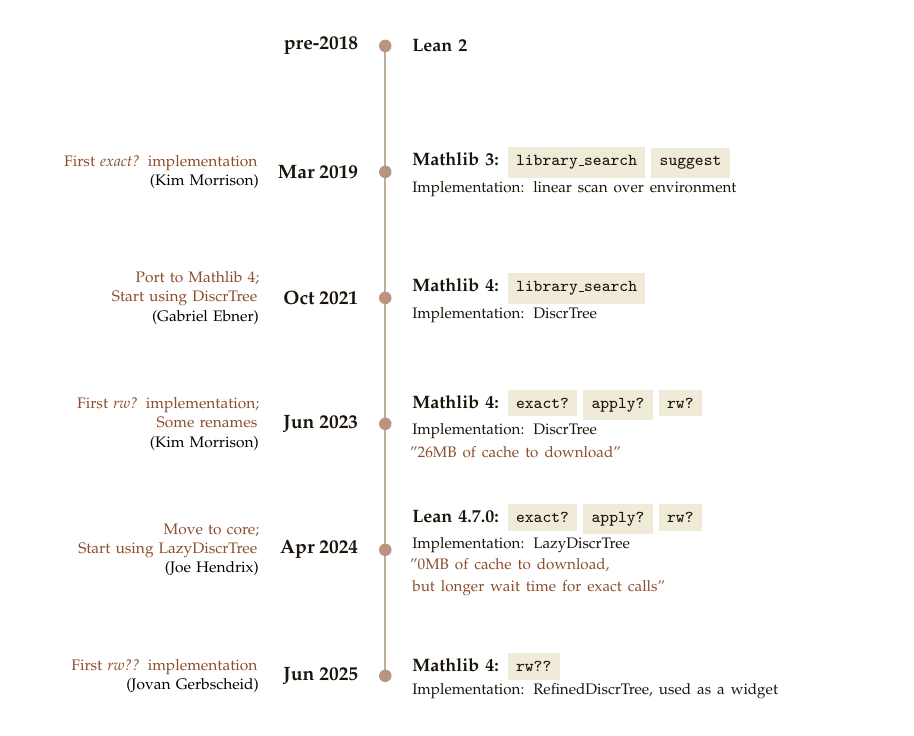
\begin{tikzpicture}[
    yr/.style    = {font=\fontsize{7}{9}\selectfont\bfseries\color{ink}, align=right},
    who/.style   = {font=\fontsize{5.5}{7}\selectfont, align=right, text width=2.8cm},
    evt/.style   = {font=\fontsize{6.5}{8}\selectfont\color{ink}, align=left, text width=5.9cm},
    dot/.style   = {circle, fill=keyterra!60, inner sep=1.6pt},
    arr/.style   = {color=inkghst, line width=0.7pt},
    auth/.style  = {font=\fontsize{5.5}{7}\selectfont\itshape\color{inkfaint}, align=center},
  ]
    % vertical spine
    \draw[color=inkghst, line width=0.6pt] (0,0) -- (0,-8.0cm);

    % --- nodes ---
    % pre-2018
    \node[dot] (d0) at (0, 0) {};
    \node[yr,  anchor=east] at (-0.22cm, 0) {pre-2018};
    \node[evt, anchor=west] at ( 0.22cm, 0) {\textbf{Lean 2}};

    % 2018
    \node[dot] (d1) at (0, -1.6cm) {};
    \node[yr,  anchor=east] at (-0.22cm, -1.6cm) {Mar 2019};
    \node[who, anchor=east] at (-1.5cm, -1.6cm) {\textcolor{keyterra}{First \textit{exact?} implementation}\\(Kim Morrison)};
    \node[evt, anchor=west] at ( 0.22cm, -1.6cm)
      {\textbf{Mathlib 3:} \colorbox{codebg}{\ttfamily\fontsize{6}{7}\selectfont library\_search} \colorbox{codebg}{\ttfamily\fontsize{6}{7}\selectfont suggest}\\[0.2pt]{\fontsize{5.5}{7}\selectfont Implementation: linear scan over environment}};

    \draw[arr] (d0) -- (d1);

    % Nov 2022
    \node[dot] (d2) at (0, -3.2cm) {};
    \node[yr,  anchor=east] at (-0.22cm, -3.2cm) {Oct 2021};
    \node[who, anchor=east] at (-1.5cm, -3.2cm) {\textcolor{keyterra}{Port to Mathlib 4;\\ Start using DiscrTree}\\(Gabriel Ebner)};
    \node[evt, anchor=west] at ( 0.22cm, -3.2cm)
      {\textbf{Mathlib 4:} \colorbox{codebg}{\ttfamily\fontsize{6}{7}\selectfont library\_search}\\[0.2pt]{\fontsize{5.5}{7}\selectfont Implementation: DiscrTree
      }
      };

    \draw[arr] (d1) -- (d2);

    % Jun 2023
    \node[dot] (d3) at (0, -4.8cm) {};
    \node[yr,  anchor=east] at (-0.22cm, -4.8cm) {Jun 2023};
    \node[who, anchor=east] at (-1.5cm, -4.8cm) {\textcolor{keyterra}{
      First \textit{rw?} implementation;  \\
      Some renames}\\(Kim Morrison)};
    \node[evt, anchor=west] at ( 0.22cm, -4.8cm)
      {\textbf{Mathlib 4:} \colorbox{codebg}{\ttfamily\fontsize{6}{7}\selectfont exact?} \colorbox{codebg}{\ttfamily\fontsize{6}{7}\selectfont apply?} \colorbox{codebg}{\ttfamily\fontsize{6}{7}\selectfont rw?}\\[0.2pt]{\fontsize{5.5}{7}\selectfont Implementation: DiscrTree\\[0.4pt]\textcolor{keyterra}{"26MB of cache to download"}}};

    \draw[arr] (d2) -- (d3);

    % Apr 2024
    \node[dot] (d4) at (0, -6.4cm) {};
    \node[yr,  anchor=east] at (-0.22cm, -6.4cm) {Apr 2024};
    \node[who, anchor=east] at (-1.5cm, -6.4cm) {\textcolor{keyterra}{Move to core;\\ Start using LazyDiscrTree}\\(Joe Hendrix)};
    \node[evt, anchor=west] at ( 0.22cm, -6.4cm)
      {\textbf{Lean 4.7.0:} \colorbox{codebg}{\ttfamily\fontsize{6}{7}\selectfont exact?} \colorbox{codebg}{\ttfamily\fontsize{6}{7}\selectfont apply?} \colorbox{codebg}{\ttfamily\fontsize{6}{7}\selectfont rw?}\\[0.2pt]{\fontsize{5.5}{7}\selectfont Implementation: LazyDiscrTree\\[0.4pt]\textcolor{keyterra}{"0MB of cache to download,\\but longer wait time for exact calls"}}};

    \draw[arr] (d3) -- (d4);

    % Jun 2025
    \node[dot] (d5) at (0, -8.0cm) {};
    \node[yr,  anchor=east] at (-0.22cm, -8.0cm) {Jun 2025};
    \node[who, anchor=east] at (-1.5cm, -8.0cm) {\textcolor{keyterra}{First \textit{rw??} implementation}\\(Jovan Gerbscheid)};
    \node[evt, anchor=west] at ( 0.22cm, -8.0cm)
      {\textbf{Mathlib 4:} \colorbox{codebg}{\ttfamily\fontsize{6}{7}\selectfont rw??}\\[0.2pt]{\fontsize{5.5}{7}\selectfont Implementation: RefinedDiscrTree, used as a widget}};

    \draw[arr] (d4) -- (d5);

  \end{tikzpicture}
  \end{center}
\end{frame}


\section{}
\begin{frame}{}
  \vfill
  \centering
  {\Large Questions}
  \vfill
\end{frame}


\end{document}
